\documentclass[10pt,a4paper]{article}
\usepackage{subcaption}
\usepackage{graphicx}

%%%%%%%%%%%%%%%%%%%%%%%%%%%
% MODIFY:

\newcommand{\authorA}{Milena Schwarz (***REMOVED***)}
\newcommand{\authorB}{Antonia Gobillard (***REMOVED***)}
\newcommand{\authorC}{Muhammed Yusuf Mermer (***REMOVED***)}
\newcommand{\authorD}{Nayeon Ahn (***REMOVED***)}
\newcommand{\authorE}{Hammad Basit (***REMOVED***)}
\newcommand{\teamlead}{~\textbf{Project lead}}
\newcommand{\groupNumber}{H} % - YOUR GROUP NUMBER
\newcommand{\exerciseNumber}{1} % - THE NUMBER OF THE EXERCISE
\newcommand{\sourceCodeLink}{\href{https://github.com/Hammad-7/MLCMS\_Exercises/tree/main/Exercise01}{https://github.com/Hammad-7/MLCMS\_Exercises/tree/main/Exercise01}}

\newcommand{\workPerAuthor}{
\authorA \teamlead& Task 1&20\%\\
      &Task 2&20\%\\
      &Task 3&20\%\\
      &Task 4&20\%\\
      &Task 5&20\%\\
      \hline
\authorB & Task 1&20\%\\
      &Task 2&20\%\\
      &Task 3&20\%\\
      &Task 4&20\%\\
      &Task 5&20\%\\
      \hline
\authorC & Task 1&20\%\\
      &Task 2&20\%\\
      &Task 3&20\%\\
      &Task 4&20\%\\
      &Task 5&20\%\\
      \hline
\authorD & Task 1&20\%\\
      &Task 2&20\%\\
      &Task 3&20\%\\
      &Task 4&20\%\\
      &Task 5&20\%\\
      \hline
\authorE & Task 1&20\%\\
      &Task 2&20\%\\
      &Task 3&20\%\\
      &Task 4&20\%\\
      &Task 5&20\%\\
}

%%%%%%%%%%%%%%%%%%%%%%%%%%%

%%
% imports for the exercise sheets
%

\usepackage[utf8]{inputenc}
\usepackage{amsmath}
\usepackage{amsfonts}
\usepackage{amssymb}

\usepackage[yyyymmdd]{datetime}
\renewcommand{\dateseparator}{--}

\usepackage[left=2cm,right=2cm,top=3cm,bottom=3cm]{geometry}

\usepackage{hyperref}

\usepackage{amsthm}
\newtheorem{lem}{Lemma}
\newtheorem{thm}{Theorem}
\newtheorem{cor}{Corollary}
\newtheorem{rem}{Remark}
\newtheorem{definition}{Definition}
\newtheorem{ter}{Terminology}

\usepackage{graphicx}

\newcommand{\M}{\mathcal{M}}
\newcommand{\N}{\mathcal{N}}
\newcommand{\K}{\mathcal{K}}
\newcommand{\SPDk}{\mathbb{P}^k}
\newcommand{\vol}{\text{vol}}

\newcommand{\Figref}[1]{Figure~\ref{#1}}
\newcommand{\figref}[1]{figure~\ref{#1}}
\newcommand{\Eqnref}[1]{Equation~(\eqref{#1})}
\newcommand{\eqnref}[1]{equation~(\eqref{#1})}

\usepackage{float}
\usepackage{tabularx}

\usepackage{fancyhdr}
\pagestyle{fancy}

\usepackage{totcount}
\newtotcounter{taskCounter}
\newtotcounter{pointCounter}
\newenvironment{task}[1]{\noindent\stepcounter{taskCounter}\textbf{Report on task #1}\smallbreak\hrule\smallbreak}{\smallbreak\hrule\bigbreak}


\title{Report for exercise \exerciseNumber~from group~\groupNumber}

\makeatletter
\let\thetitle\@title
\let\theauthor\@author
\let\thedate\@date
\makeatother

\providecommand{\versiondate}{\today}

\lhead{Exercise sheet \exerciseNumber}
\chead{Master Praktikum: Modelling and Simulation of Crowds WS2019/20}
\rhead{TUM}
\lfoot{Report of Group \groupNumber}
\cfoot{\thepage}
\rfoot{Last compiled: \versiondate}
\renewcommand{\headrulewidth}{0.4pt}
\renewcommand{\footrulewidth}{0.4pt}

\newcommand{\frontpage}{
\begin{center}
\textbf{\thetitle}\\~\\
\end{center}
\begin{table}[H]
\begin{tabular}{ll}
Tasks addressed:&\total{taskCounter}\\
Authors:&\authorA\\
&\authorB\\
&\authorC\\
&\authorD\\
&\authorE\\
Last compiled:&\versiondate\\
Source code:&\sourceCodeLink
\end{tabular}
\end{table}
\vfill
The work on tasks was divided in the following way:
\begin{table}[H]
\begin{tabularx}{\textwidth}{X|p{2cm}|p{2cm}}
\workPerAuthor
\end{tabularx}
\end{table}
\newpage
}

\begin{document}

\frontpage

\begin{task}{1, Setting up the modeling environment}

In the first task, the main goal is setting up the modeling environment which the following tasks depend on. 
We have undertaken a revision and enhancement of the 'ExampleGUI' program for better functionality and User Experience. 
We used the 'Place' method to design the window in \verb|tkinter| \cite{tkinter}. The place method allows you to position a widget within a specified frame by directly entering x and y coordinate values. We used this method because it is useful to precisely position a widget and we will constantly change the size of the grid(widgets). (x= x-coordinate, y= y-coordinate) to set the position.\\

Here is a breakdown of the features and functionalities that are included:

\begin{enumerate}
  \item Step Simulation Button: This feature allows users to incrementally advance through the simulation timeline. By pressing this button, the user can observe the progression of the simulation step by step.
  \item Restart Simulation Button: Should there be a need to revert to the initial state of the simulation, users can utilize this button. Upon pressing, it resets the entire simulation to its default state.
  \item Run Simulation Button: With the help of this feature, the user can watch the entire simulation without the need to repeatedly advance through the timeline themselves.  
  \item Create Scenario Button: Activating this button spawns an additional window, as depicted in the provided illustration. Within this window, users have the capability to:
  \begin{itemize}
      % \item Construct a grid.
      \item Introduce pedestrian elements.
      \item Incorporate obstacles.
      \item Designate destinations.
  \end{itemize}
  \item Load Scenario Button: For users who have predefined simulation settings saved as JSON files, this button facilitates the importing of those scenarios into the current session.
  \item Save Scenario Button: Post-simulation or during its configuration, users might want to preserve the current scenario for future reference or use. This button empowers users to save the present simulation scenario as a JSON file.
\end{enumerate}

The \verb|restart_scenario| function corresponding to the 'Restart Simulation' Button simply loads the file of the current running scenario again. \\ 
Within the function \verb|run_simulation| the already existing function \verb|step_scenario| was used. Between each function call, the program waits 0.05 seconds due to the usage of \verb|time.sleep| \cite{time}. \\

% description of constructing a grid within the following create scenario description
In order for the user to intuitively create a new scenario, multiple options can be presented. We decided that this functionality should be a part of the Graphical User Interface (GUI). A consideration is to let the user draw pedestrians, targets, and obstacles with the mouse. The downside to this idea is that, especially with large grids, the input would be imprecise. Hence, we created a new window in which the user can write explicit integers. \\
The function \verb|popupwin| creates and shows a simple user interface with multiple labels, entries, and buttons. The user can set a new scenario size, as well as add pedestrians, targets, and obstacles. All of this can happen due to the \verb|add_more| function. The function adds one pedestrian, one target, and one obstacle at maximum. After clicking the corresponding button, the newly added objects can be seen in the main window, and the entries have been cleared with the \verb|clear_entries| function in order to make it possible to add more of each desired object. In figure \ref{fig:createSimulationGUI} new objects locations are set to be added. After clicking the "add more" button, the new objects can be seen on the left side of figure \ref{fig:createSimulationError} in the main window. It includes error handling for numbers too small or too big for the scenario size, in which case an error messagebox, provided by \verb|tkinter|, appears to explain to the user which inputs are possible, as can be seen in figure \ref{fig:createSimulationError}. \\ 

This choice of User Interface provides various advantages: the user can see changes fast and problems with entries can easily be related to the last input. Additionally, there is no need to continuously change the Interface, e.g. with a plus button, in order to fit more cells to add multiple objects of the same kind at once. After the creation of the new scenario, the finish button closes the additional window with the help of the \verb|close_win| function, and the user can save the scenario. \\

The \verb|load_scenario| and \verb|save_scenario| functions benefit from the \verb|filedialog| of \verb|tkinter|. This enables the user to select any JSON file on the computer as well as save new scenarios with the desired title and location. 

\begin{figure}[H]
     \centering
     \begin{subfigure}[b]{0.8\textwidth}
         \centering
         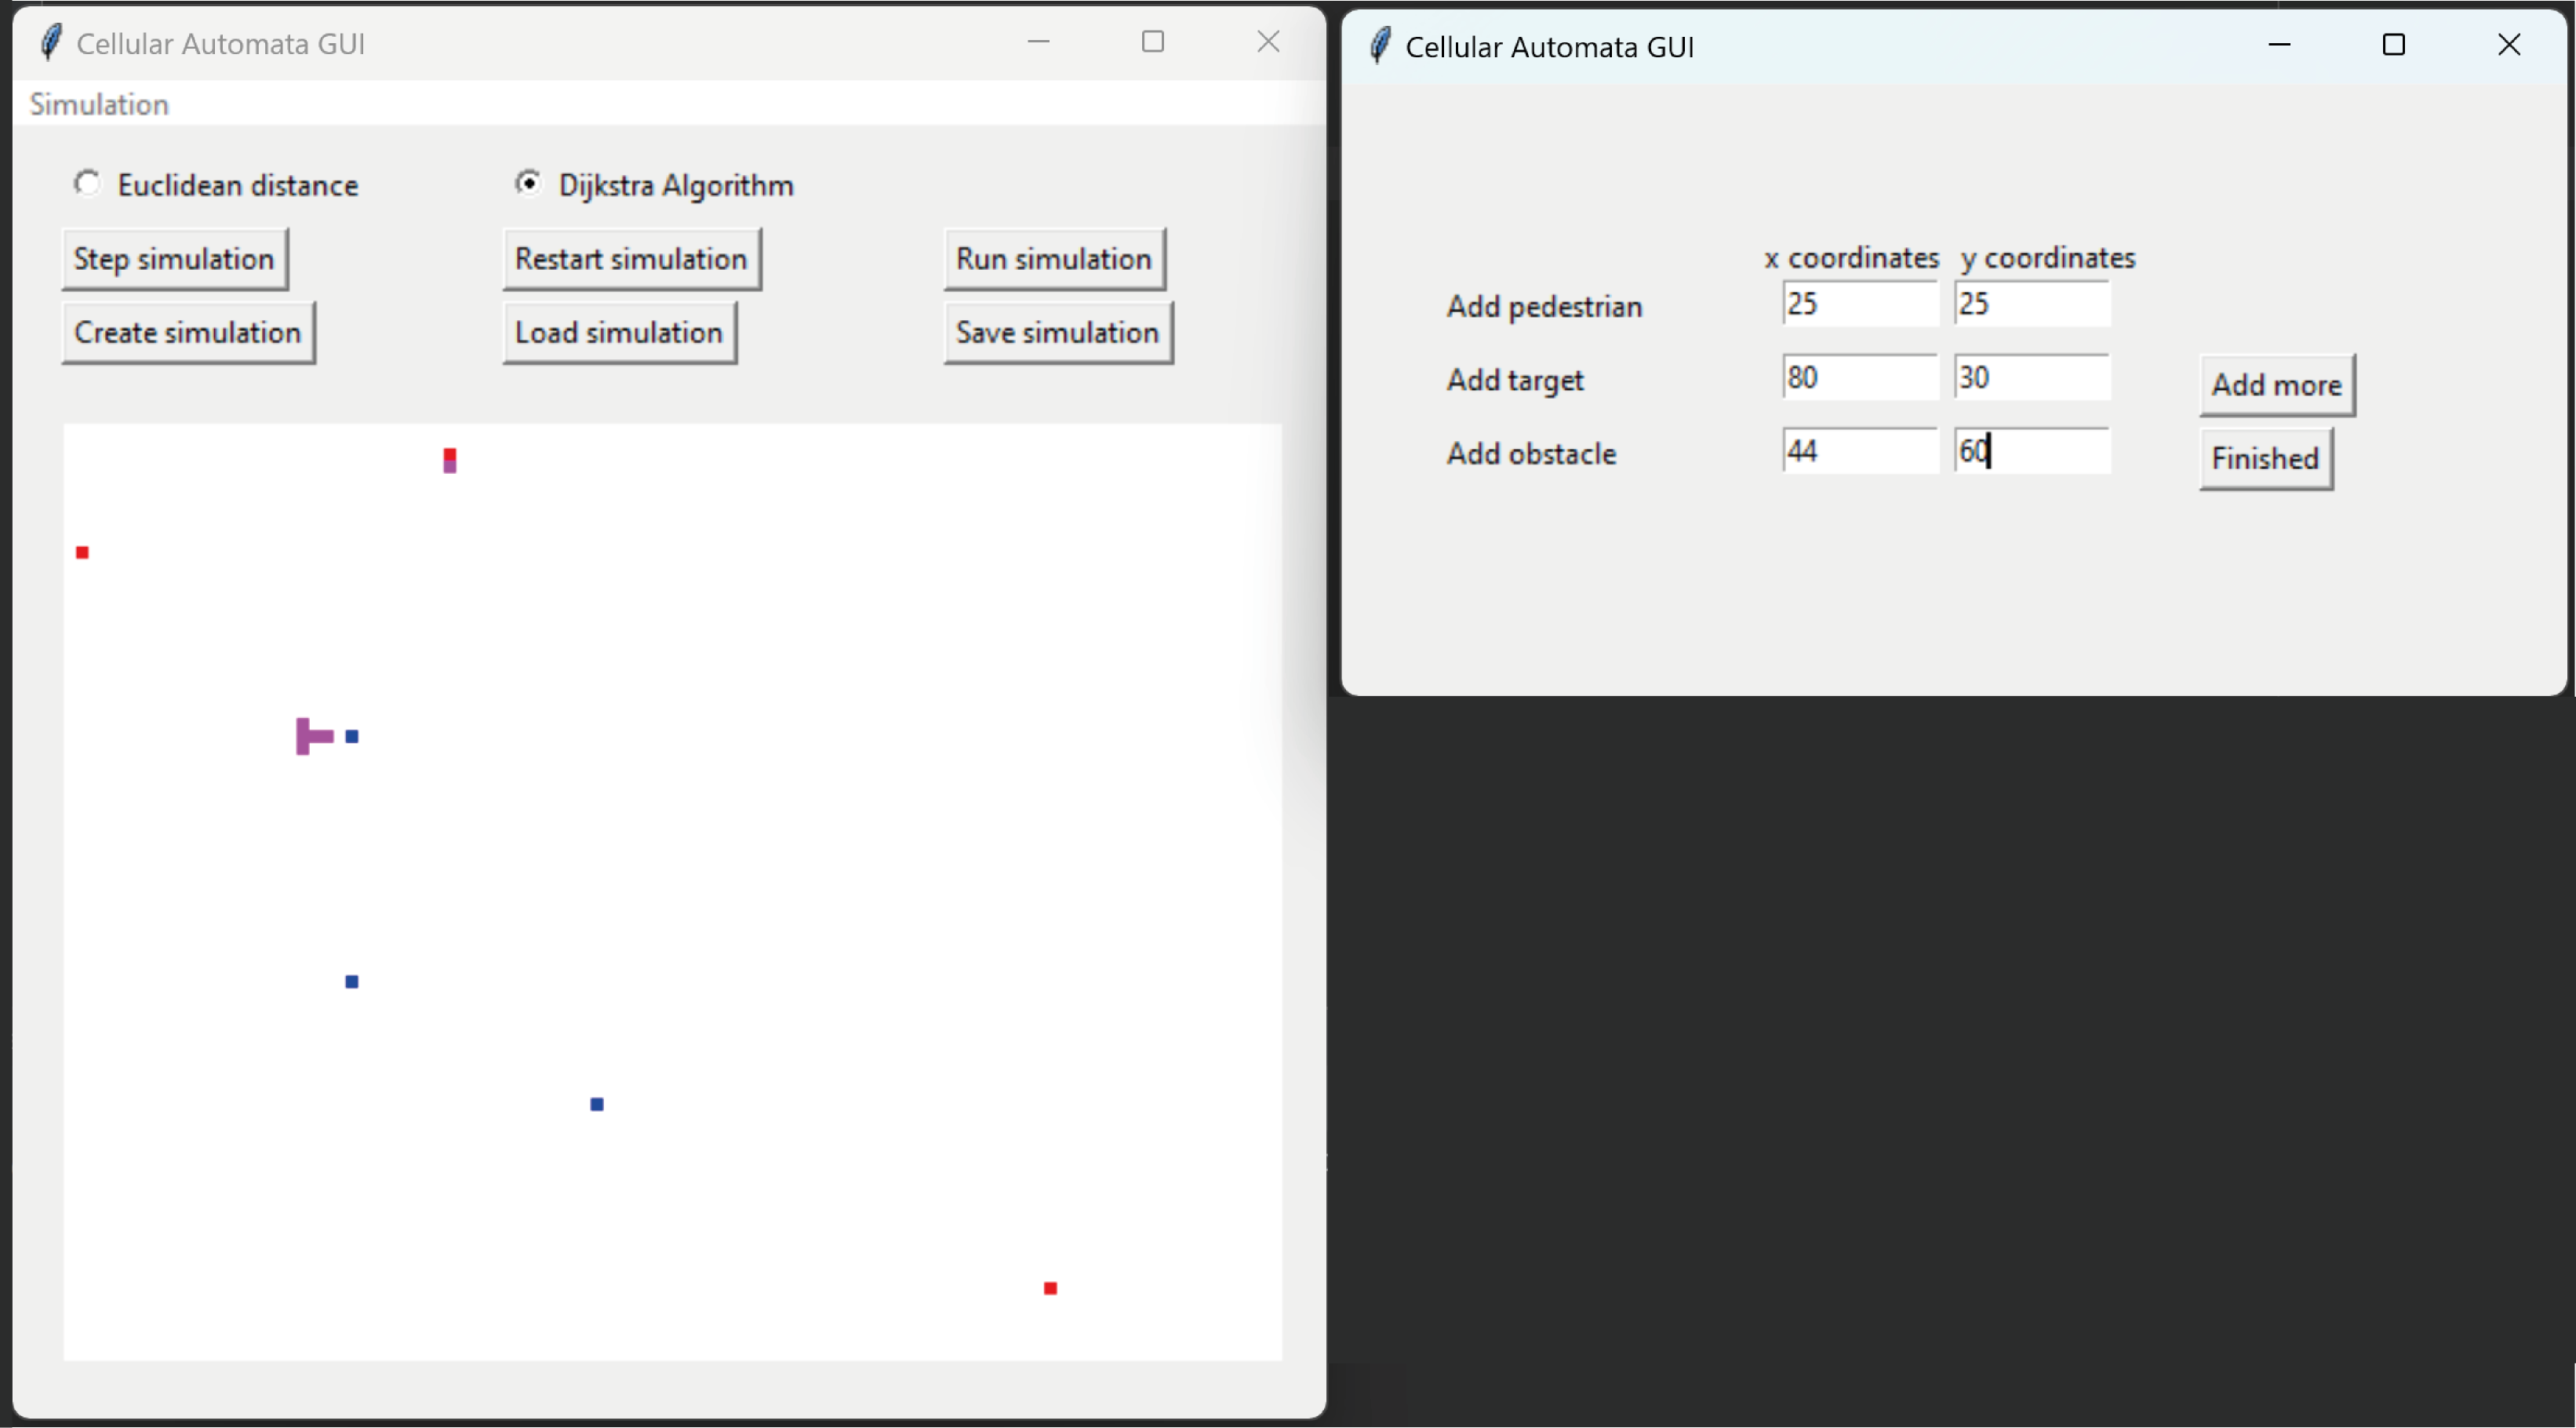
\includegraphics[width=\textwidth]{images/1-create simulation gui.png}
         \caption{Create simulation GUI}
         \label{fig:createSimulationGUI}

         \centering
         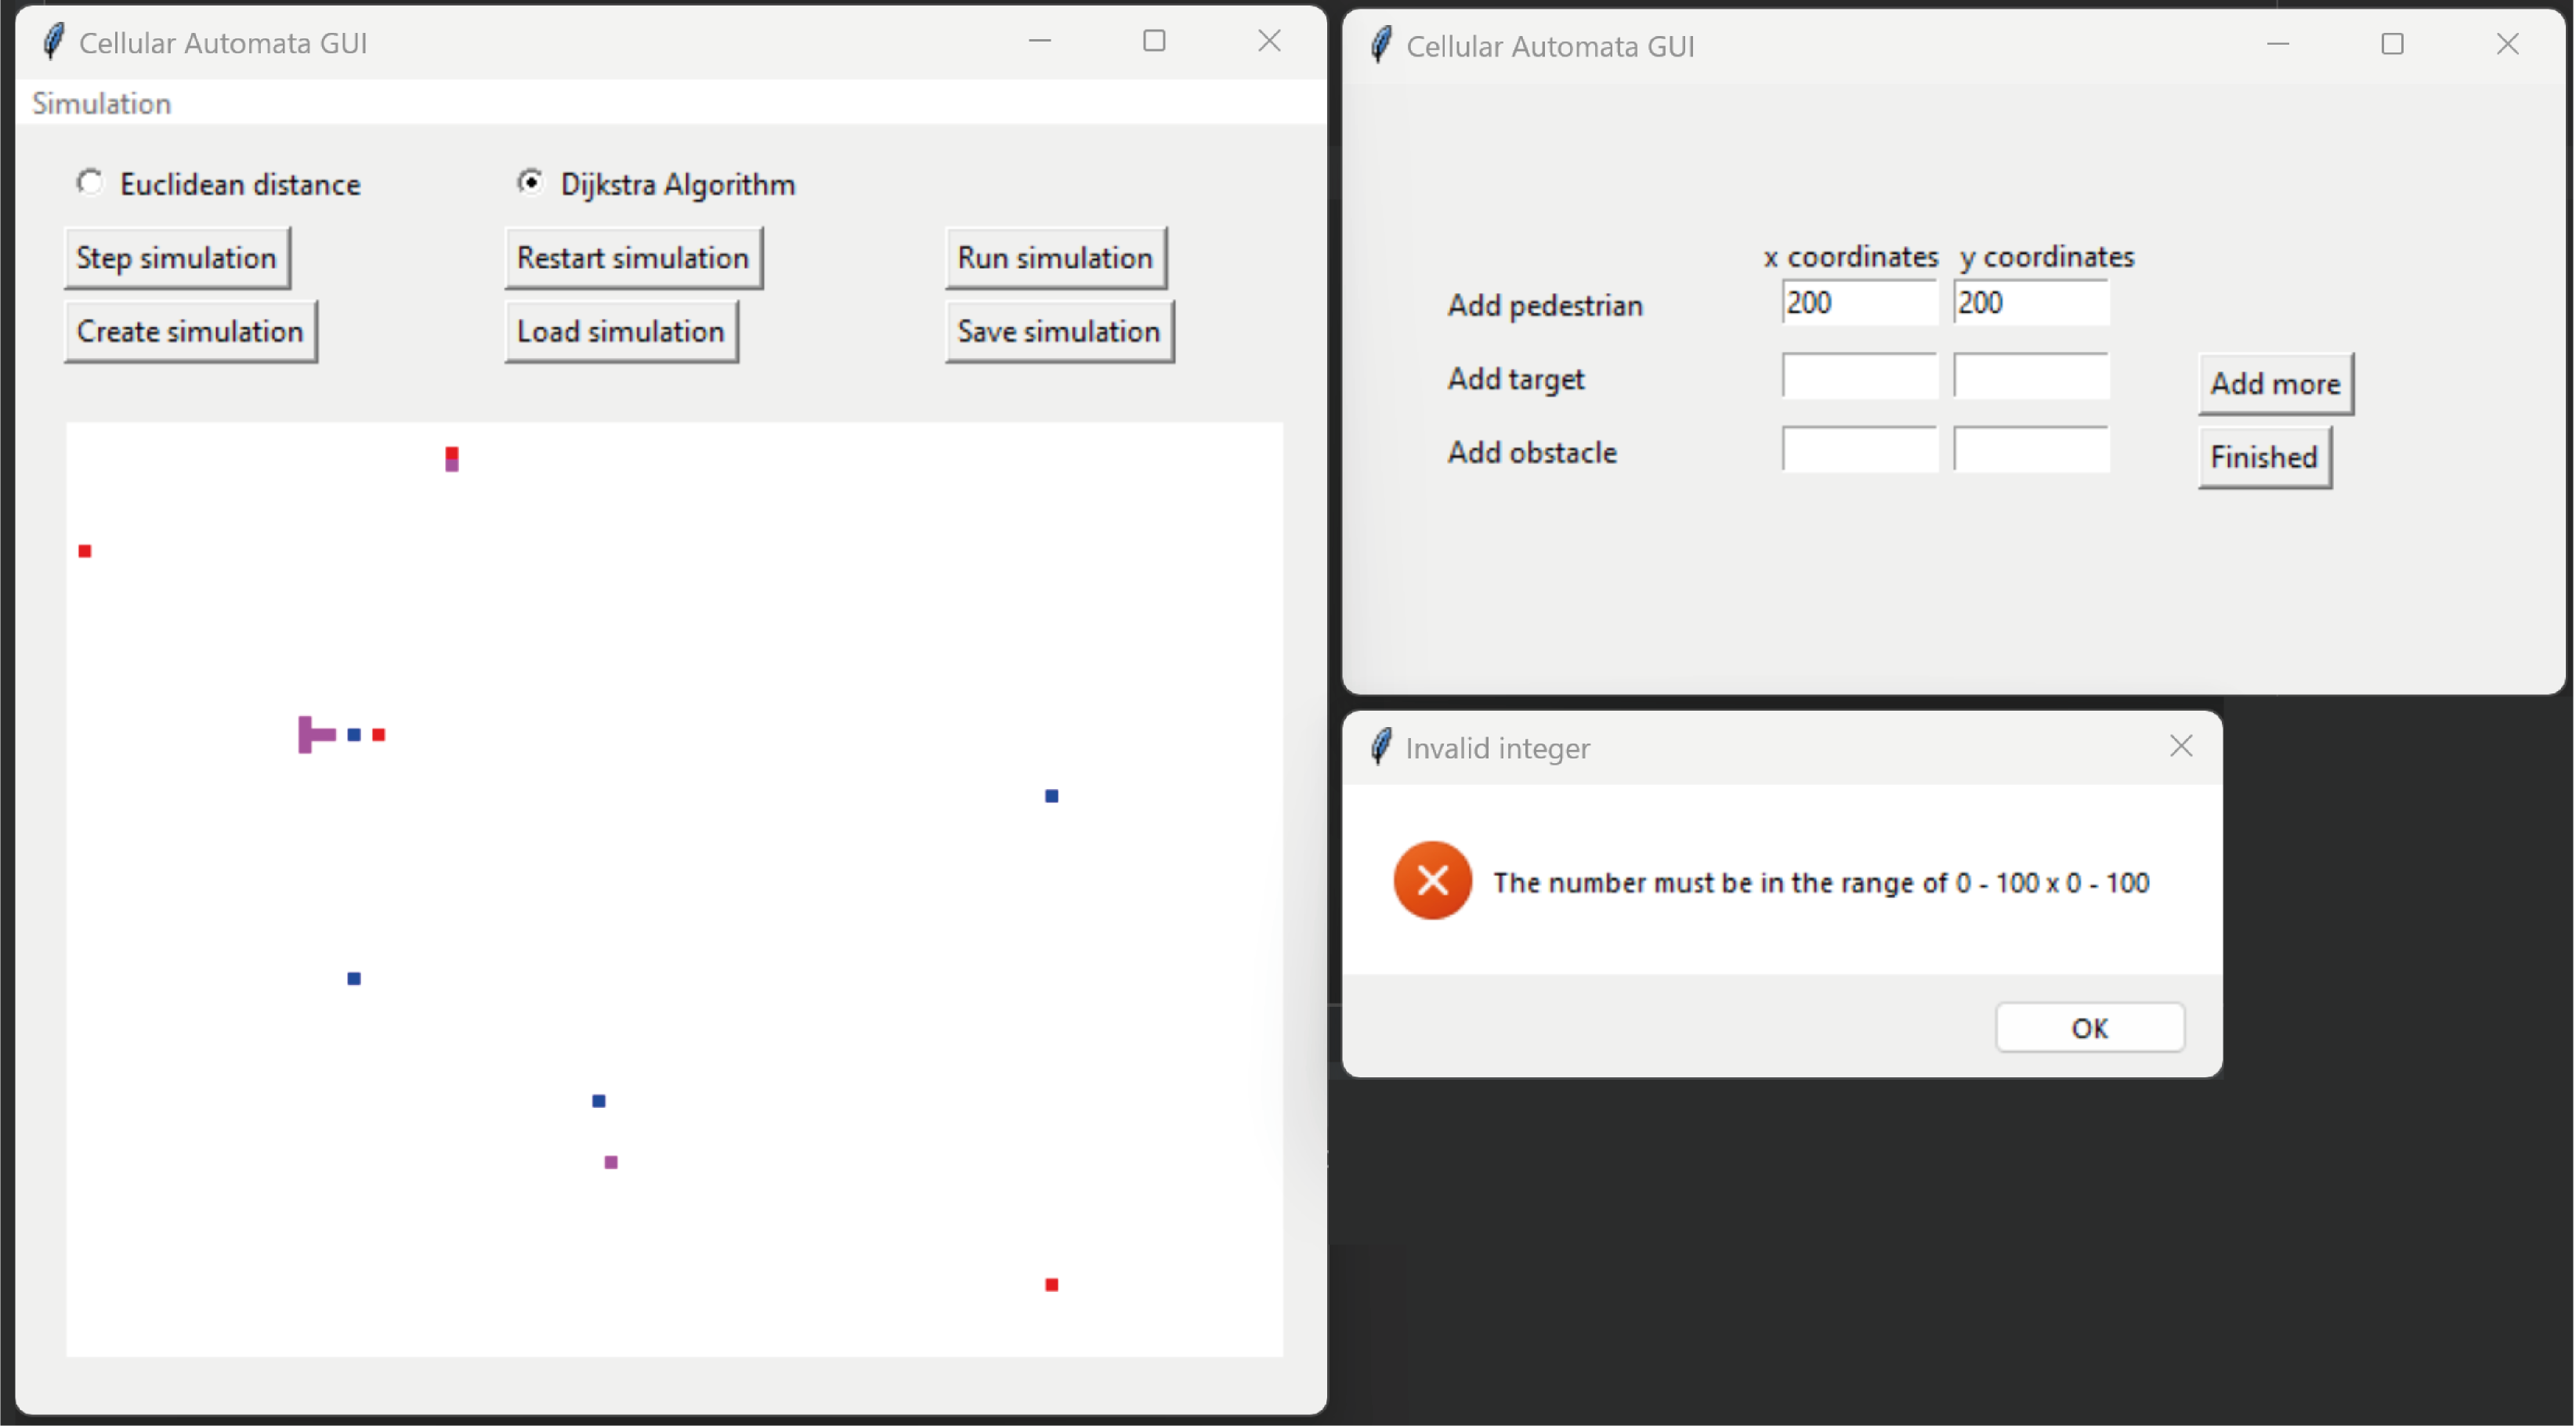
\includegraphics[width=\textwidth]{images/1-invalid integer error.png}
         \caption{Error Messagebox}
         \label{fig:createSimulationError}
     \end{subfigure}
    \caption{The GUI for creating a new simulation includes entry fields and buttons to add pedestrians, targets, and obstacles to the current grid}
    \label{fig:createSimulation}
\end{figure}

\end{task}

\newpage
\begin{task}{2, First step of a single pedestrian}
For this task, we provide an input JSON file with a scenario consisting of 50 by 50 cells (2500 in total). The pedestrian is at the coordinate (5,25), whereas the target is 20 cells away at the coordinate (25,25). \\

\begin{figure}[H]
 \centering
 \begin{subfigure}[b]{0.4\textwidth}
     \centering
     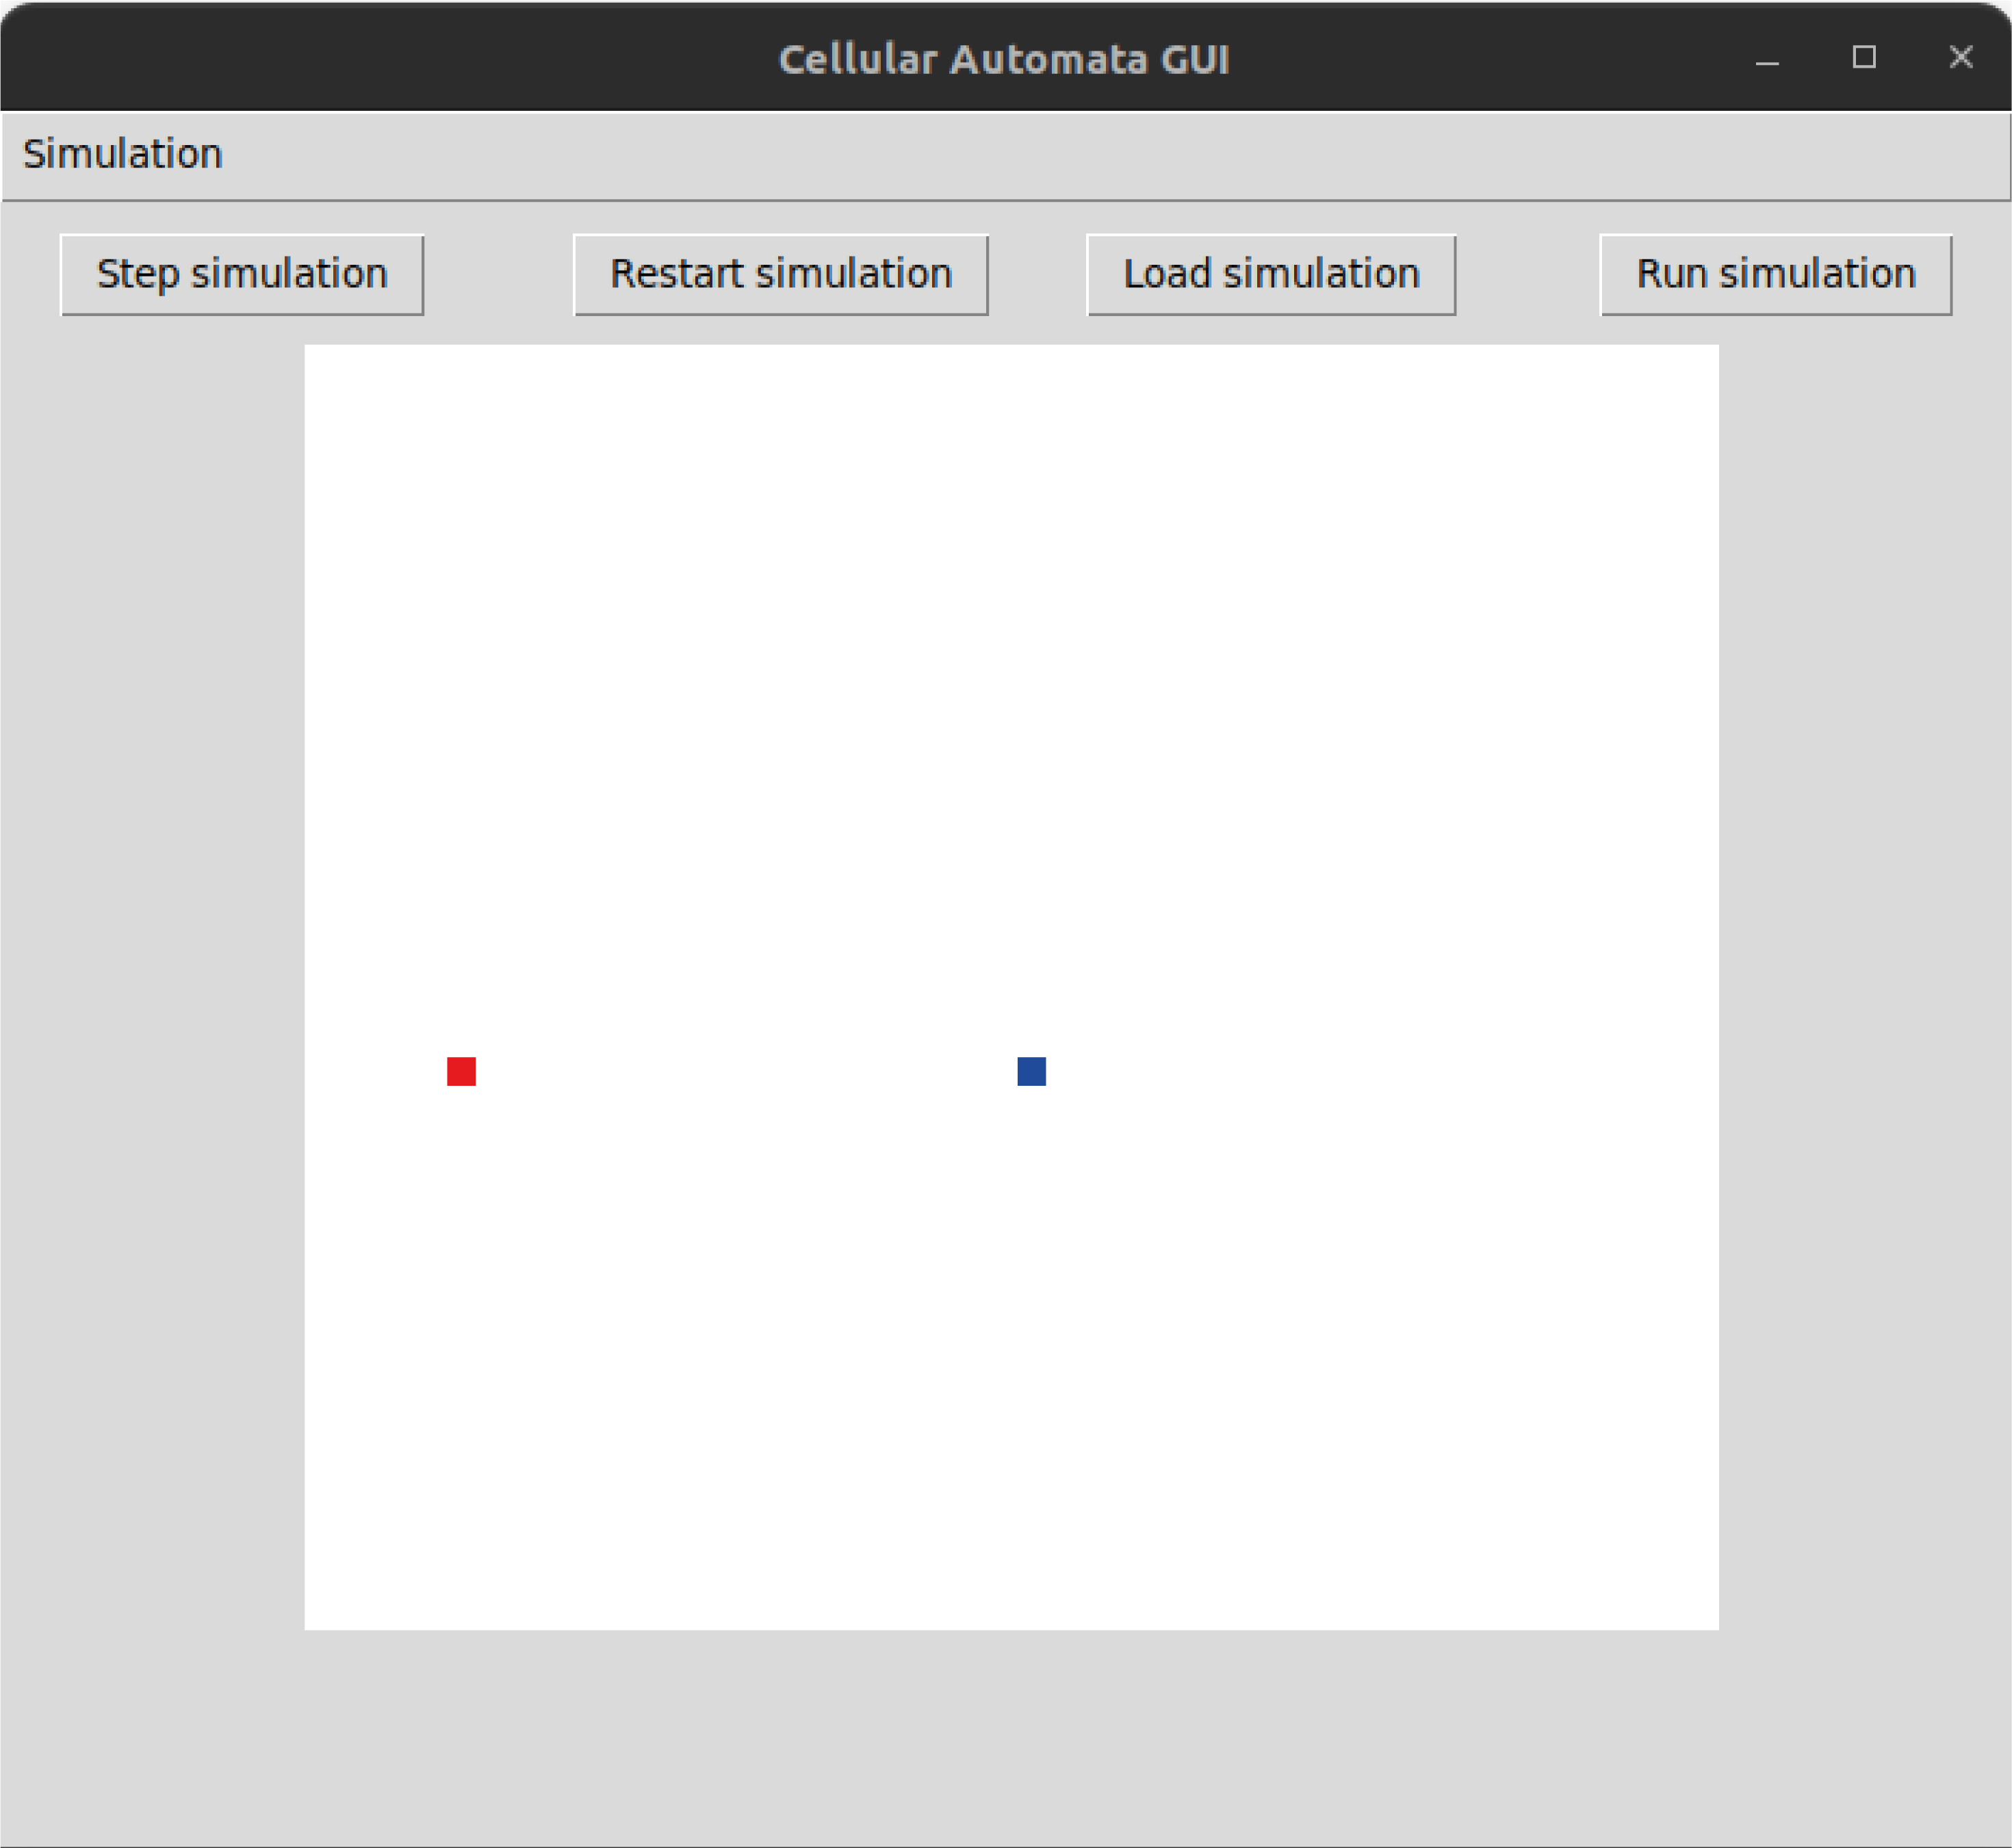
\includegraphics[width=\textwidth]{images/scenario2_initial.png}
    \caption{Initial configuration of the scenario 2}
    \label{fig:scneario2_initial}
 \end{subfigure}
 \begin{subfigure}[b]{0.4\textwidth}
      \centering
     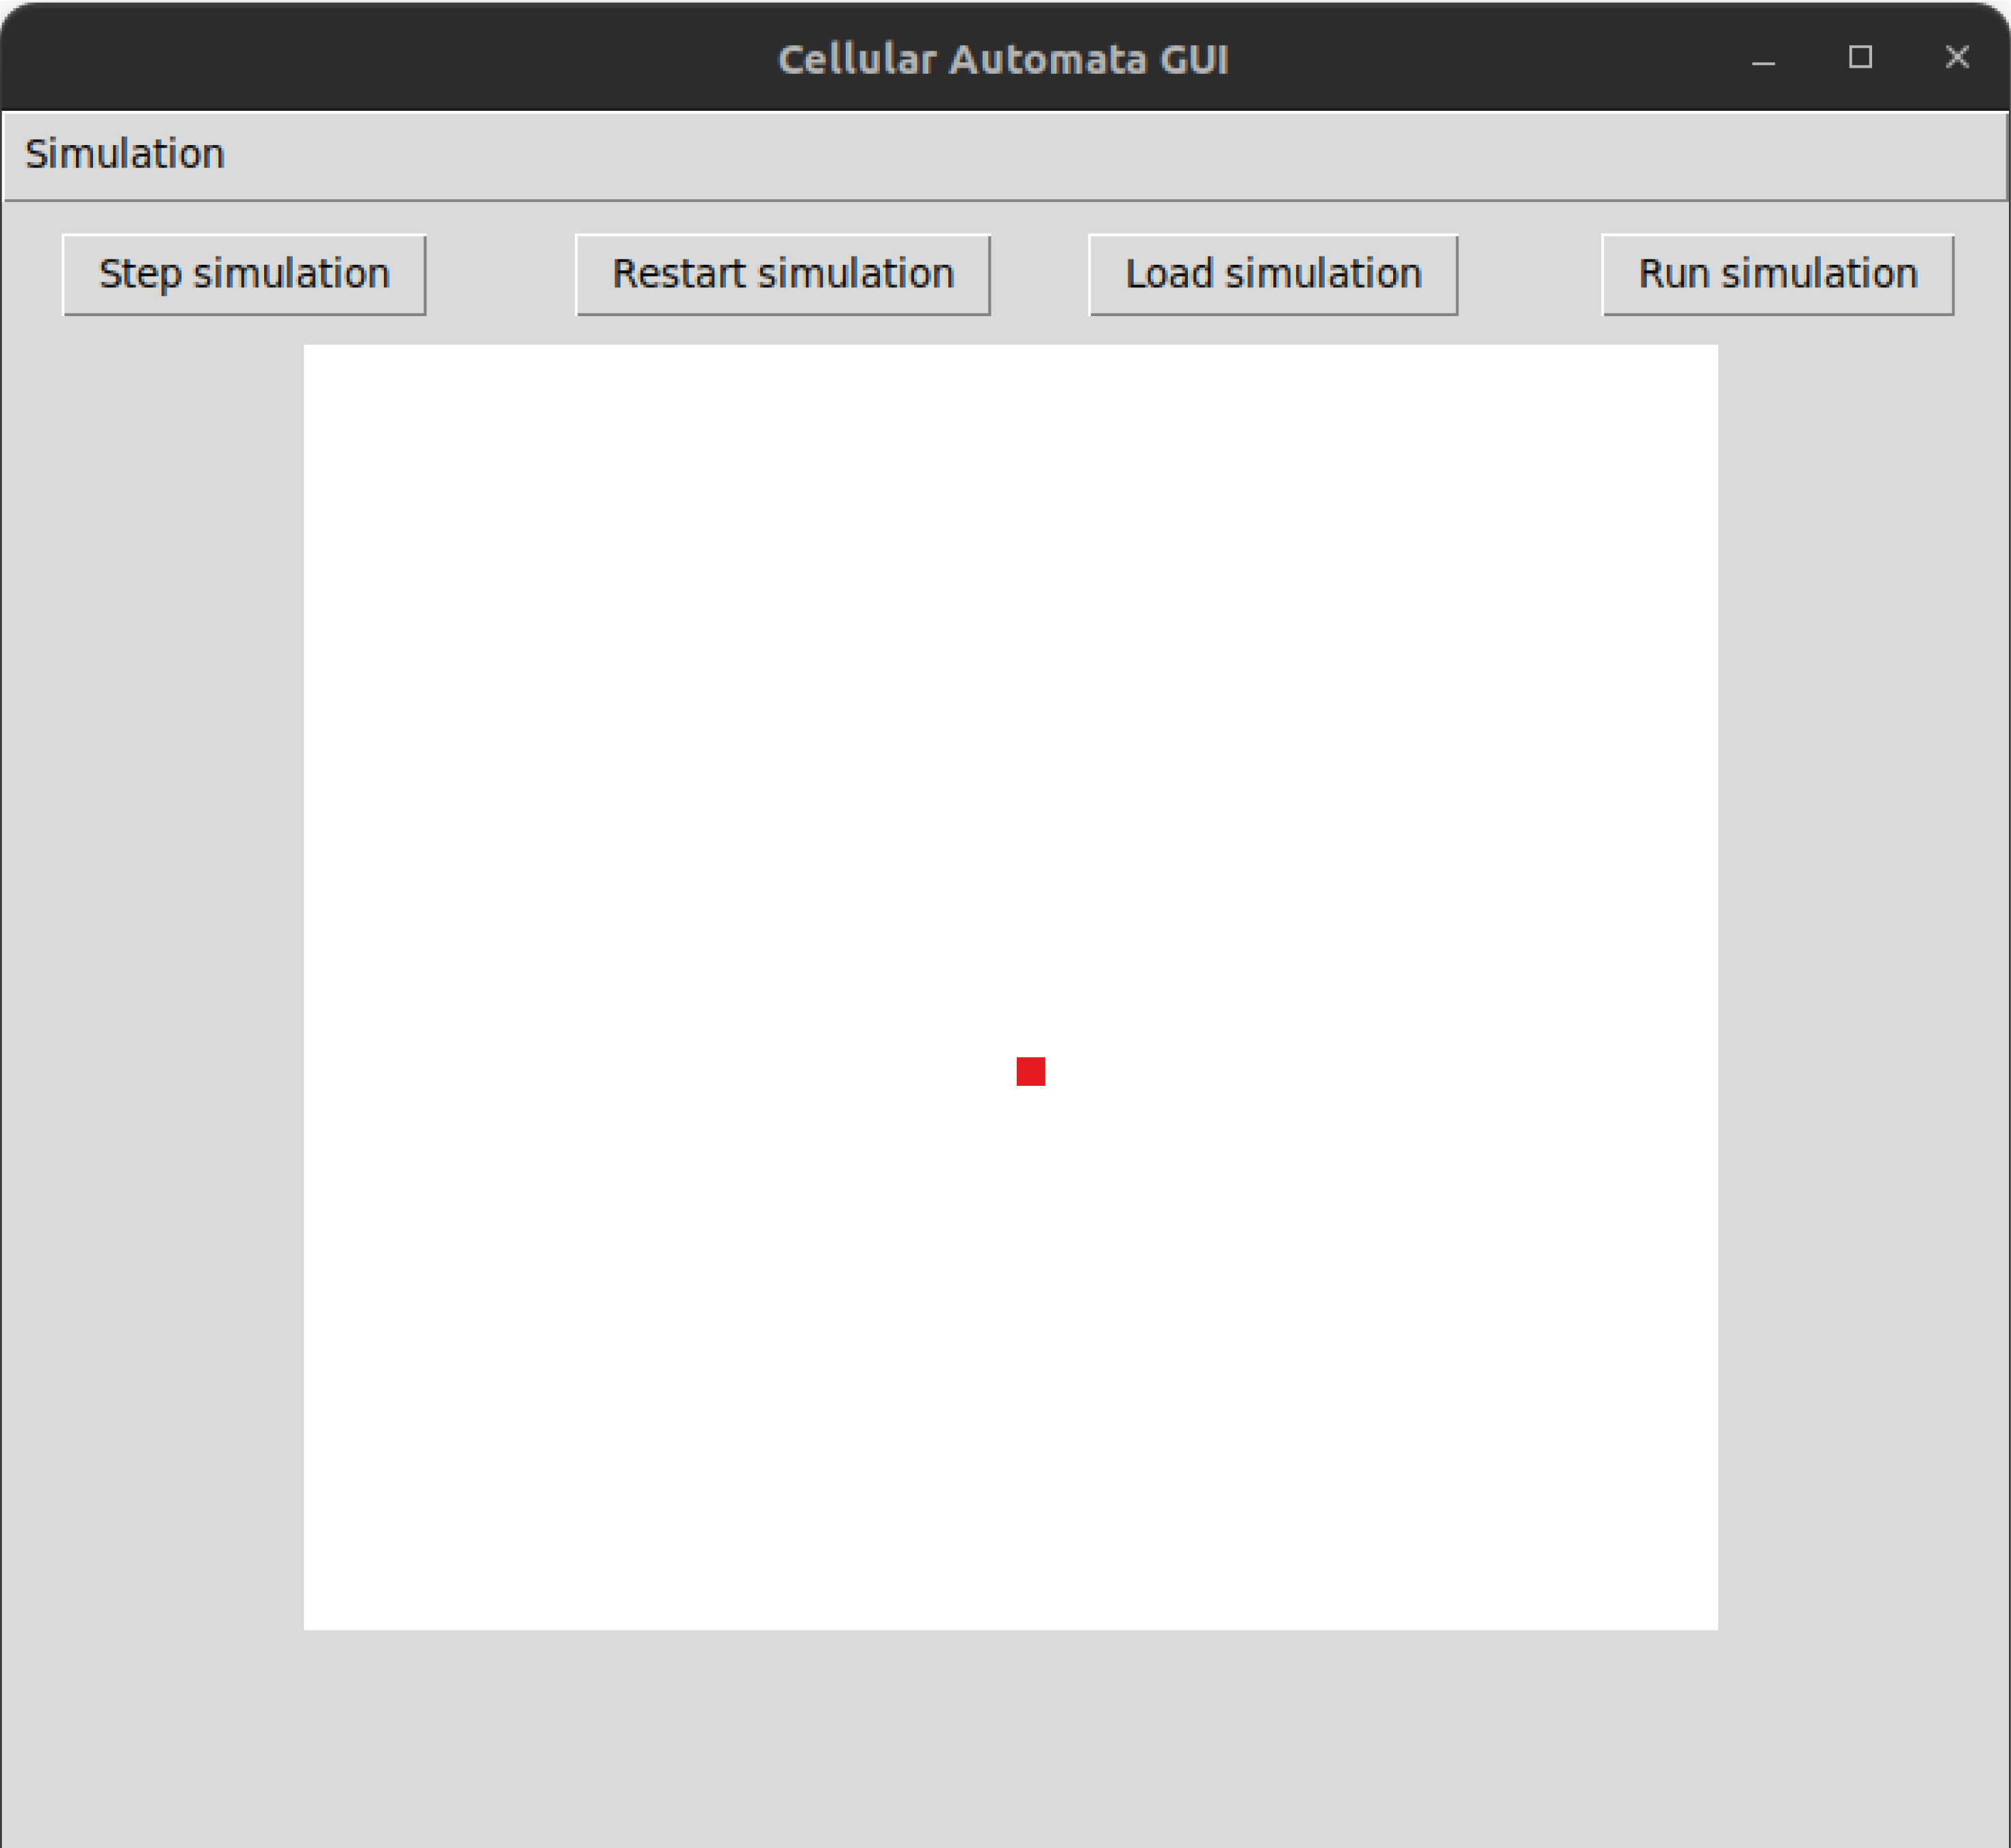
\includegraphics[width=\textwidth]{images/scenario2_final.png}
     \caption{Final configuration of the scenario 2}
     \label{fig:scneario2_final}
 \end{subfigure}
\end{figure}

Figure \ref{fig:scneario2_initial} shows the initial configuration of scenario 2 on the grid.  Figure \ref{fig:scneario2_final} shows the final output after simulating the scenario for 25 time steps. The pedestrian reaches the target in 20 time steps and waits there for 5 seconds until the simulation is completed.

\end{task}

\begin{task}{3, Interaction of pedestrians}
For this scenario, 5 pedestrians are now placed at roughly equal distances from the centered target. The input file for this task is the \verb|scenario3.json|. We take a grid of 80 by 80 cells (6400 in total) and have the target centered at the coordinate (40,40). The pedestrians are placed roughly at 30 meters distances at the following coordinates from the target: 
\begin{itemize}
    \item (15, 22)
    \item (34, 9)
    \item (68, 28)
    \item (59, 64)
    \item (14, 55)
\end{itemize}

Figure \ref{fig:scenario3_initial} shows the initial setup of the grid with the pedestrians and the targets. \\
\begin{figure}
 \centering
 \begin{subfigure}[t]{0.4\textwidth}
    \centering
     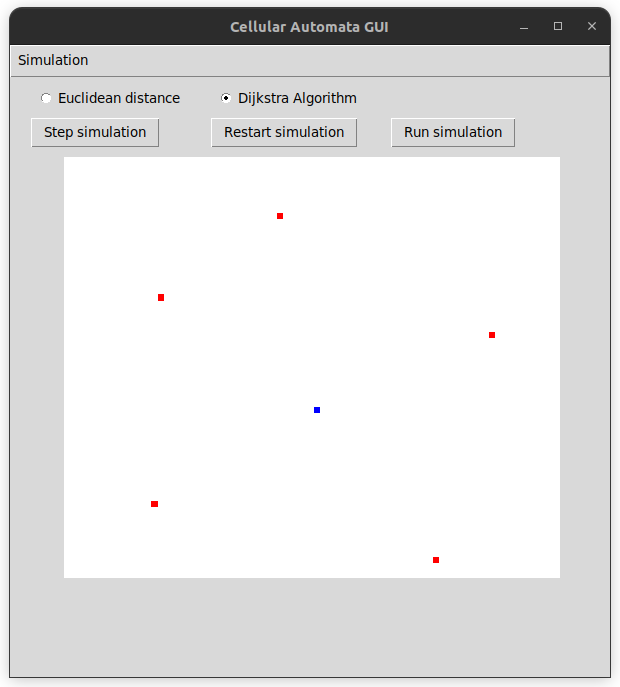
\includegraphics[width=\textwidth]{images/scenario3_intial.png}
     \caption{Initial configuration of scenario 3 \\ }
     \label{fig:scenario3_initial}
 \end{subfigure}
 \begin{subfigure}[t]{0.4\textwidth}
     \centering
     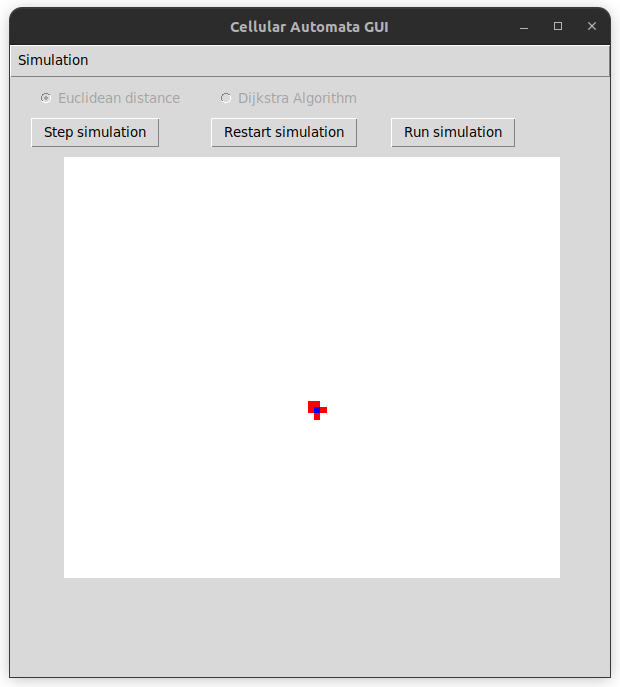
\includegraphics[width=\textwidth]{images/scenario3_final.png}
     \caption{Final configuration of scenario 3 \\ before being absorbed by target}
     \label{fig:scenario3_final}
 \end{subfigure}
\end{figure}

When employing solely the Euclidean distance as the metric, it was observed that elements moving diagonally reached the target more quickly compared to those moving along horizontal or vertical paths. This expedited arrival occurs due to pedestrians covering a greater distance (approximately $\sqrt{2}$ units) while traversing diagonally, as opposed to only 1 unit when moving vertically or horizontally. \\

To address this discrepancy, we introduced the concept of waiting time. Pedestrians are made to wait longer to simulate a real-life scenario by incorporating a waiting period equivalent to $\sqrt{2}$ seconds when they move diagonally. Conversely, a waiting duration of 1 second is imposed when they move in horizontal or vertical directions. This adjustment equalizes the arrival times of all pedestrians at the target, ensuring that they reach it almost simultaneously, regardless of their chosen path. \\

Result: Figure \ref{fig:scenario3_final} shows the configuration of scenario 3 just before the pedestrians are absorbed by the target. All the pedestrians reach roughly at equal times as they are placed at roughly equal distances from the center.
\end{task}

\begin{task}{4, Obstacle avoidance}
For previous parts, Euclidean distance was a very good method to implement distance for determining the motion of the pedestrians as there is no limitation such as obstacles or height on the direct path to influence to direction of the pedestrians. They just follow the shortest path to the target point without any angle problem. However in real life: 


\begin{quote}
``Nothing is as easy as it looks'' - Murphy's Law
\end{quote}  

There are obstacles that we need to consider. For part 4, using simply Euclidean distance is not fine, as one cannot go through objects and needs another path. Let us first take a look into what will happen when we use rudimentary obstacle avoidance.\\

Rudimentary obstacle avoidance employed the calculation of Euclidean distance. In this method, pedestrians would navigate towards to the targets linearly. However, we advanced it so that pedestrians will not traverse through objects, but this does not mean that they will just stop without trying other ways. They can look at their surrounding environment and walk around the obstacle if the barrier is not that big.\\

To do this, we have improved the \texttt {update\_euclidean\_move} function within \texttt {scenario\_elements.py}. Normally, at the next update, the Euclidean distance needs to be shorter than the current one. However, our current code only tries to look at the shortest distance among the neighbours, it does not compare them with the current one. Therefore, when pedestrians are stopped by an obstacle, even though their movement will increase their distance to the obstacle compared to the current point, pedestrians can pass to the shortest distanced neighbour of its current location, and if there is no other object in front of them, they can just beat around the object with this method. This algorithm is visualised in figure \ref{fig:task4_euc}. \\



\begin{figure}[H]
\begin{subfigure}[t]{0.5\textwidth}
 \centering
 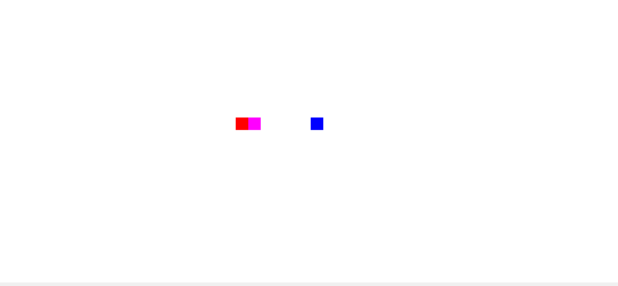
\includegraphics[width=0.5\textwidth]{images/task4_1object_touched.png}
 \caption{When pedestrian encounters an object}
 
 \end{subfigure}
\begin{subfigure}[t]{0.5\textwidth}
 \centering
 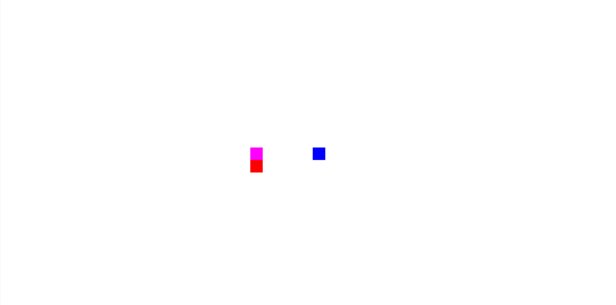
\includegraphics[width=0.5\textwidth]{images/task4_1object_passing.png}
 \caption{Even though it is longer in distance, the pedestrian tries to use its neighbours to pass the object}
 \end{subfigure}

 
\begin{center}   
\begin{subfigure}[t]{0.5\textwidth}
 \centering
 
\includegraphics[width=0.5\textwidth]{images/task4_1object_passedpng.png}
 \caption{Pedestrian passes object successfully}
 \end{subfigure}
\end{center}
\caption{Rudimentary obstacle avoidance using Euclidean distance}
 \label{fig:task4_euc}
\end{figure}

Although it could be seen as a solution, it only works for small objects that pedestrians can skip with one step. Hence, if the object is bigger and cannot be passed via one movement, the pedestrians will turn back to their first location where they first encountered the object. Then, they will twist around left and right points without successfully reaching the targets. This can be seen in figure \ref{fig:task4_eucfault}.
\\


\begin{figure}[H]
\begin{subfigure}[t]{0.5\textwidth}
 \centering
 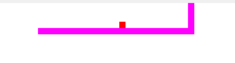
\includegraphics[width=0.5\textwidth]{images/task4_1object_touched_dummy.png}
 \caption{A pedestrian encounters an object}
 
 \end{subfigure}
 \hspace{1em}
\begin{subfigure}[t]{0.5\textwidth}
 \centering
 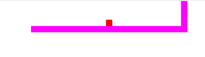
\includegraphics[width=0.45\textwidth]{images/task4_1object_passing_dummy.png}
 \caption{Even though it is longer in distance, the pedestrian tries to use its neighbours to pass the object.} 
 \end{subfigure}
 
\begin{center}   
\begin{subfigure}{0.5\textwidth}
 \centering
 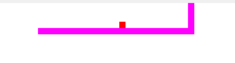
\includegraphics[width=0.5\textwidth]{images/task4_1object_notpassed_dummy.png}
 \caption{The pedestrian could not pass the object and starts to twist around left-right points and cannot reach any target}

 \end{subfigure}
\end{center}
\caption{Rudimentary obstacle avoidance fails}
 \label{fig:task4_eucfault}
\end{figure}

If we use this implementation on the chicken test scenario in which there is a U-shaped obstacle between the pedestrian and the target, we will see similar results. The pedestrian, trapped inside this box-shaped obstacle, is unable to exit or proceed towards the target. It changes its place but nevertheless, it cannot get out of the box to reach the target point, as depicted in figure \ref{fig:task4_eucchick}. \\ 



\begin{figure}[H]
\begin{subfigure}{0.5\textwidth}
 \centering
 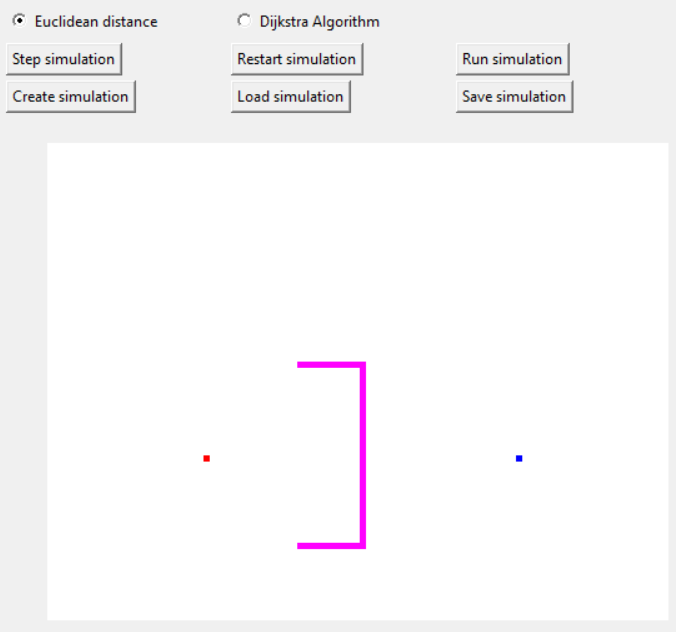
\includegraphics[width=1\textwidth]{images/task4_chicken_start.png}
 \caption{Initial setup of the chicken test}
 
 \end{subfigure}
 \hspace{1em}
\begin{subfigure}{0.5\textwidth}
 \centering
 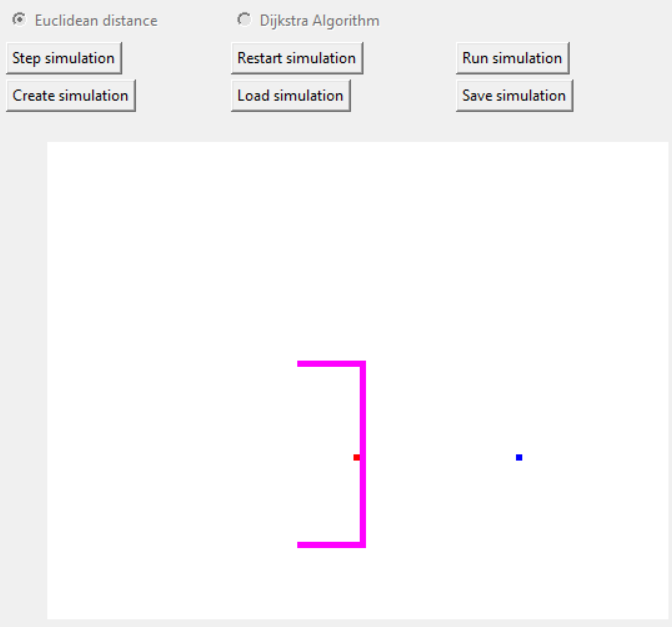
\includegraphics[width=1\textwidth]{images/task4_chicken_first_contact.png}
 \caption{The pedestrian makes contact with the obstacle} 
 \end{subfigure}
 
\begin{center}   
\begin{subfigure}{0.5\textwidth}
 \centering
 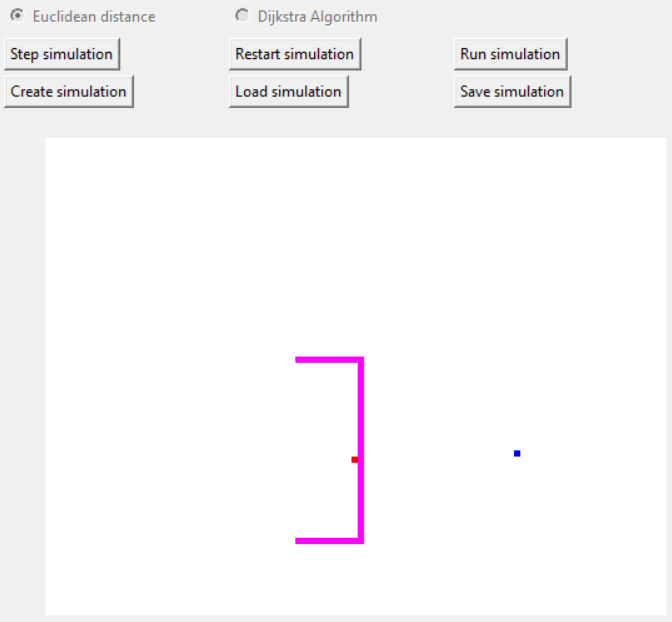
\includegraphics[width=1\textwidth]{images/task4_chicken_second_contact.png}
 \caption{The pedestrian slides to the right but still cannot pass through the object. Therefore, it will start to twist inside the object}

 \end{subfigure}
\end{center}
\caption{Chicken test fails for rudimentary obstacle avoidance}
 \label{fig:task4_eucchick}
\end{figure}

As we can indicate from these results, using rudimentary obstacle avoidance generally is not effective. Therefore, we needed to focus and explore much more effective algorithms. \\

Dijkstra's algorithm is well-suited to our objectives. In the Dijkstra algorithm, we initially assigned the cost of target points as 0, since one does not need to spend time and energy to reach these points. Then, we look at the nearest points and assign them a cost of 1. And then, we take a look at these points' neighbours and give them cost as 2. At each iteration, we try to look at the neighbours of the point with the lowest cost that has unchecked neighbours and the increment the for its neighbors by 1. This procedure is summarized in figure \ref{fig:task4_dijmod} for better understanding.\\

\begin{figure}[H]
\begin{subfigure}{0.5\textwidth}
 \centering
 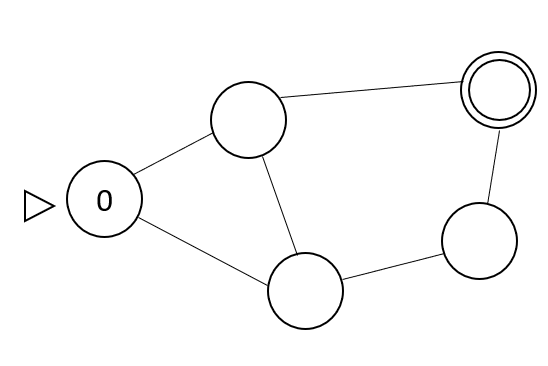
\includegraphics[width=1\textwidth]{images/task4_dij_mod_0.png}
 \caption{Initial cost at the target point is 0, \\ the cost of the other points is still unknown}
 
 \end{subfigure}
\begin{subfigure}{0.5\textwidth}
 \centering
 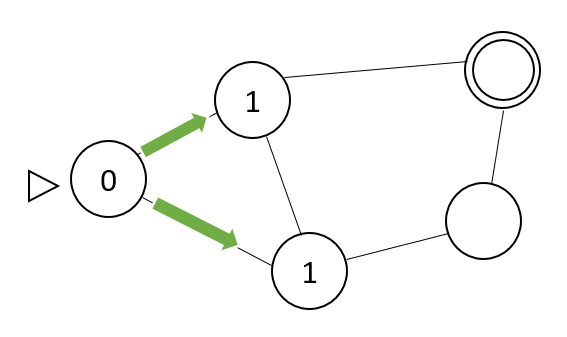
\includegraphics[width=1\textwidth]{images/task4_dij_mod_1.png}
 \caption{Looking at the neighbours of the point with the smallest cost. In this situation, it is the target point. } 
 \end{subfigure}

 
   \begin{center}
       

\begin{subfigure}{0.6\textwidth}
 \centering
 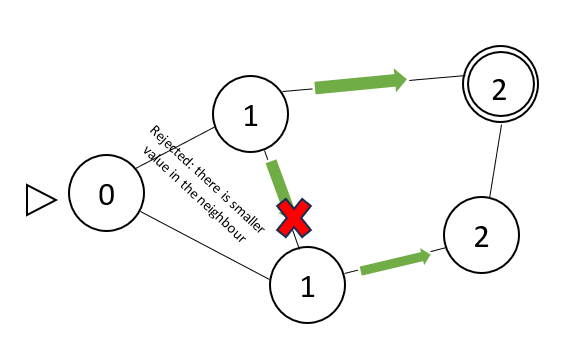
\includegraphics[width=1\textwidth]{images/task4_dij_mod_2.png}
 \caption{Looking at the neighbours of the point with the smallest cost. We already looked at the target point, therefore it is time to take a look at the next smallest points.}

 \end{subfigure}
   \end{center}

   
\begin{center}
    

\begin{subfigure}{0.8\textwidth}
 \centering
 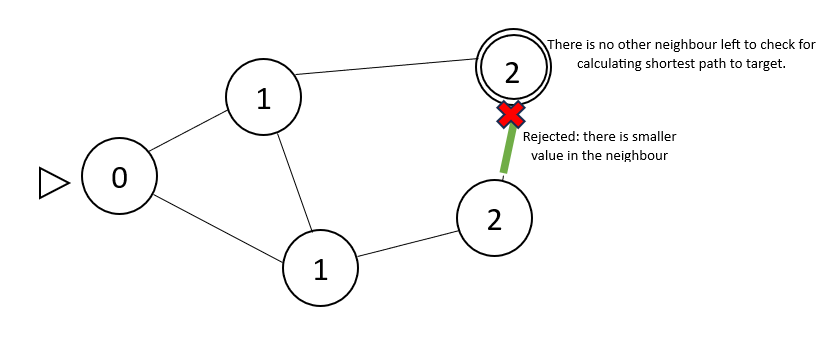
\includegraphics[width=1\textwidth]{images/task4_dij_mod_3.png}
 \caption{The end result}
 
 \end{subfigure}
 \end{center}

\caption{Example of how to use Dijkstra's algorithm}
 \label{fig:task4_dijmod}
\end{figure}

Given that our navigation domain for pedestrians is in 2D plane, we used Dijkstra's algorithm in a matrix framework. For each integer-valued coordinate point on the grid, we calculated the cost with the same method.

We provided an example for the scenario in figure \ref{fig:task4_dij2D}:





\begin{figure}[H]

\begin{center}
    

\begin{subfigure}{0.65\textwidth}
 \centering
 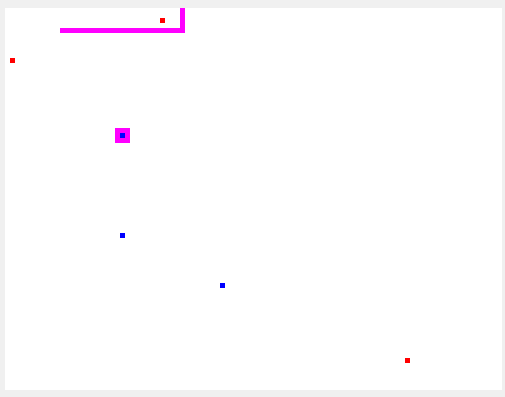
\includegraphics[width=1\textwidth]{images/task4_dij_2d.png}
 \caption{The setup of the scenario. There are 3 pedestrians and 3 targets but one of the targets is fully covered by an obstacle. }
 \end{subfigure}
 
\begin{subfigure}{0.65\textwidth}
 \centering
 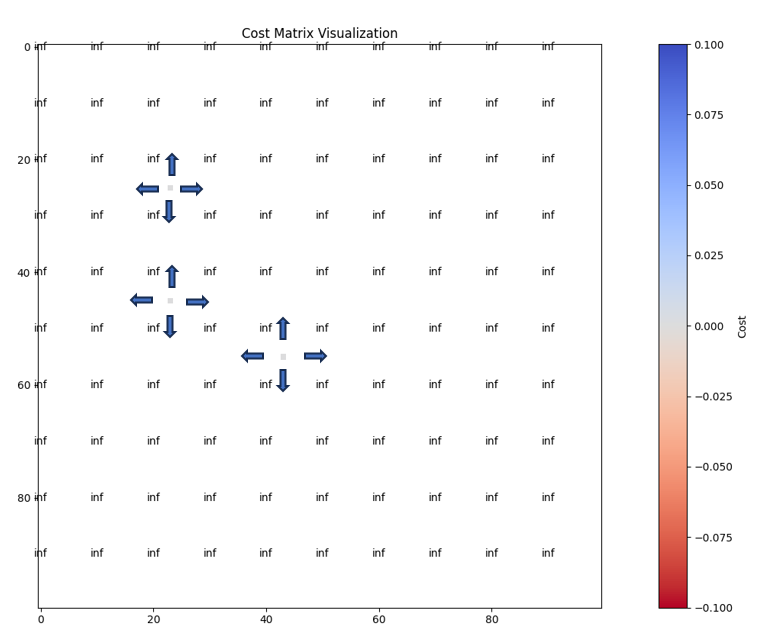
\includegraphics[width=1\textwidth]{images/task4_dij_2d_very_start.png}
 \caption{Visualization of \texttt{cost\_matrix}: Starting from target points (whose costs are 0), we will look at their neighbours and determine their respective costs.} 
 \end{subfigure}

 \end{center}

\caption{Visualization of \texttt{cost\_matrix} for a random test scenario}

\end{figure}
 
\begin{figure}[H] \ContinuedFloat


\begin{center}
    

\begin{subfigure}{0.65\textwidth}
 \centering
 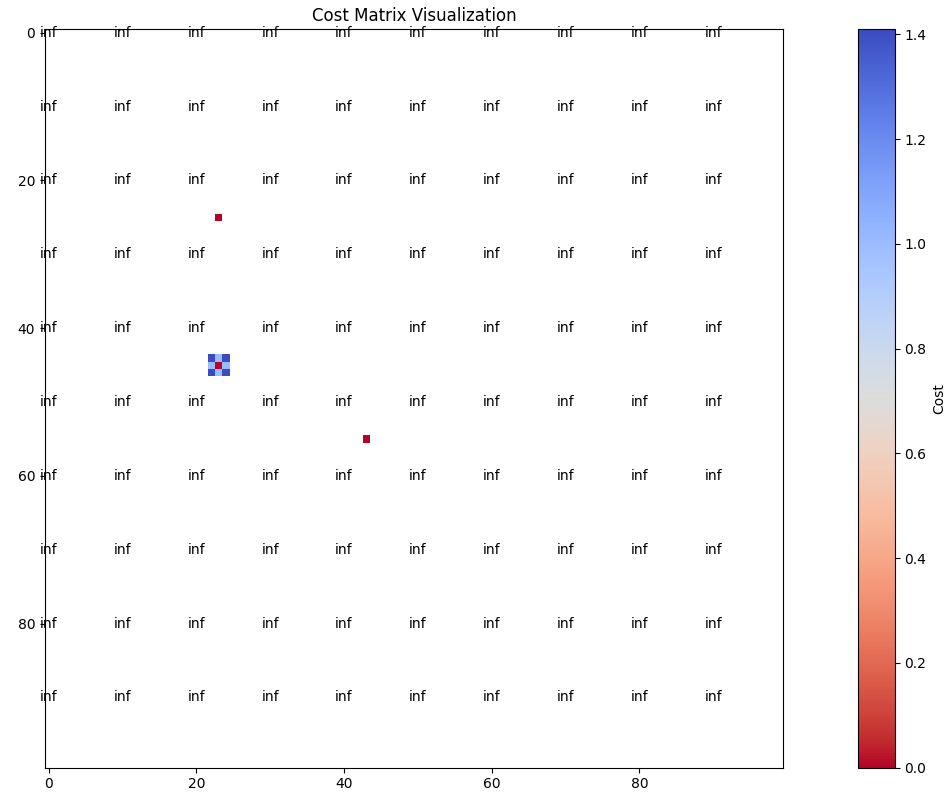
\includegraphics[width=1\textwidth]{images/task4_dij_2d_start.png}
 \caption{Visualization of \texttt{cost\_matrix}:
 Our matrix starts to expand. Even though the cost is very small near the target point, currently \texttt{matplotlib} displays them in blue. This will qualitatively change with the gain of more cost values.
 }
 \end{subfigure}

\begin{subfigure}{0.65\textwidth}
 \centering
 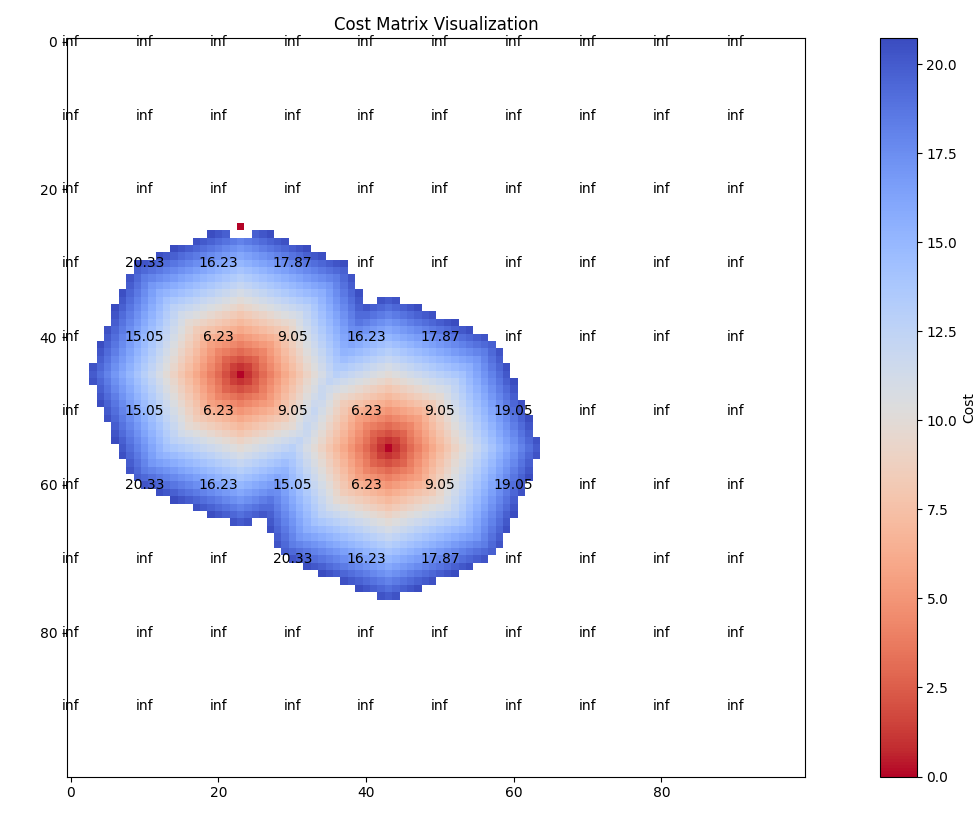
\includegraphics[width=1\textwidth]{images/task4_dij_2d_expanding.png}
 \caption{Visualization of \texttt{cost\_matrix}: It can be seen that there is no expansion from point (23,25), pictured in red, because obstacles are not considered as neighbours and thus, you cannot reach that target point from anywhere.}
 \end{subfigure}

\end{center}


\caption{Visualization of \texttt{cost\_matrix} for a random test scenario}

\end{figure}
 
\begin{figure}[H] \ContinuedFloat

\begin{center}


\begin{subfigure}{0.65\textwidth}
 \centering
 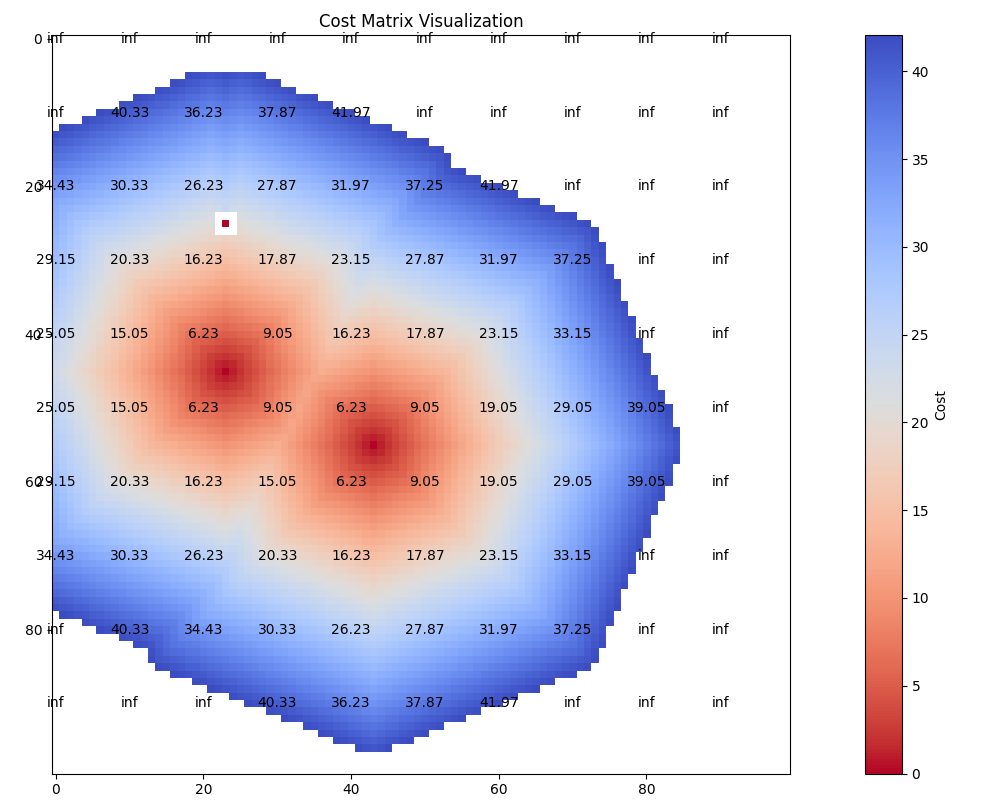
\includegraphics[width=1\textwidth]{images/task4_dij_2d_expanding2.png}
 \caption{Visualization of \texttt{cost\_matrix}: The expansion continues to large distances and cost increases as well. Therefore, points close to the target point become more red rather than blue.}
 \end{subfigure}




\begin{subfigure}{0.65\textwidth}
 \centering
 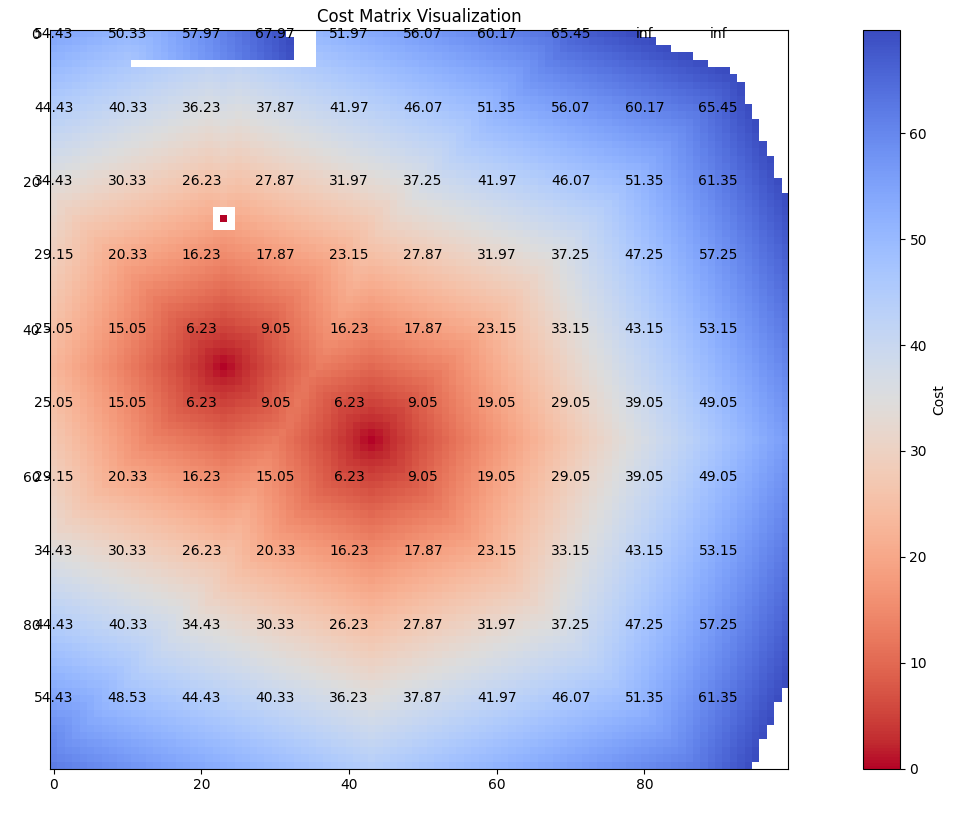
\includegraphics[width=1\textwidth]{images/task4_dij_2d_expanding3.png}
 \caption{Visualization of \texttt{cost\_matrix}: There is an L-shaped obstacle on top of the grid, therefore Dijkstra's algorithm needs to work its way around starting from the open side on the left. This is why points further inside of the L-shaped obstacle have a larger cost than the ones outside.   }
 \end{subfigure}
\end{center}

\caption{Visualization of \texttt{cost\_matrix} for a random test scenario}
\end{figure}
 
\begin{figure}[H] \ContinuedFloat
\begin{center}
    

\begin{subfigure}{0.65\textwidth}
 \centering
 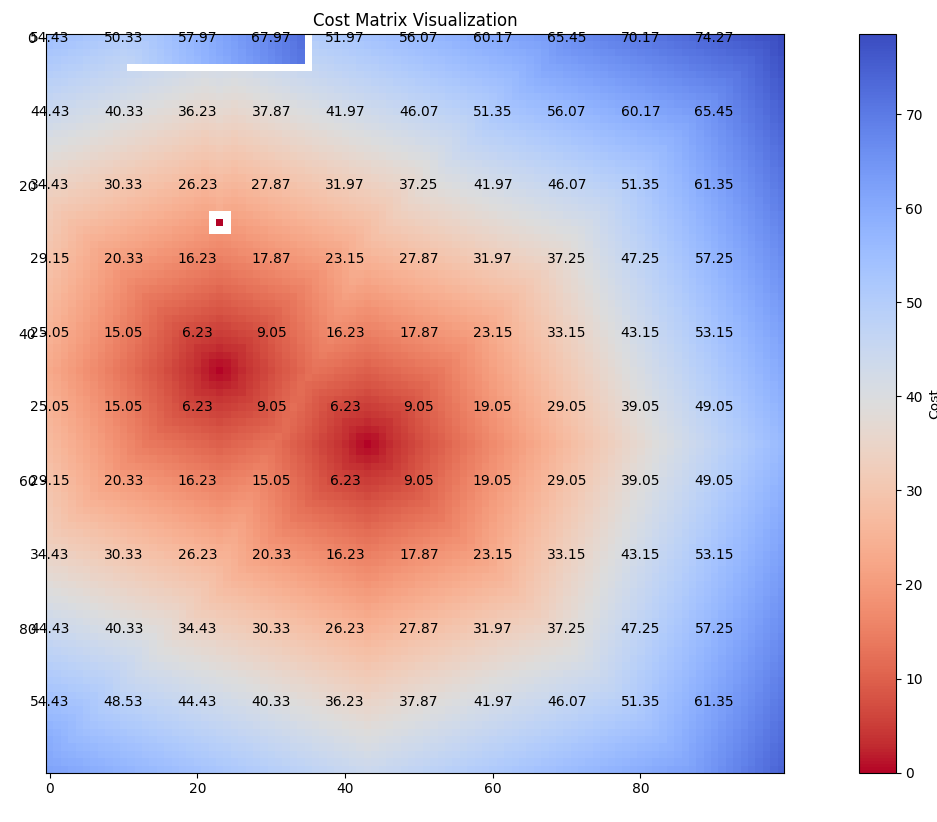
\includegraphics[width=1\textwidth]{images/task4_dij_2d_full.png}
 \caption{The final \texttt{cost\_matrix} using Dijkstra's algorithm}
 \end{subfigure}
\end{center}


\caption{Visualization of \texttt{cost\_matrix} for a random test scenario}
 \label{fig:task4_dij2D}
\end{figure}



This method works fine, but it is relatively slow compared to Euclidean distance, especially for large matrices. This was primarily due to one big reason. After looking at the neighbours of a point, our algorithm is not only looking at the next unobserved point with the lowest cost, but it looks at the cost of all neighbours of neighbours recursively. Therefore, with this method, we are looking at the same point several times which decreases our algorithm's performance significantly. \\

Subsequently, following our research and thinking, we found a way to increase performance, we can use \texttt{PriorityQueue} \cite{Queue} whose time complexity is $O(n  \cdot log n)$, compared to our first approach of time complexity $O(n^2)$.

Basically, \texttt{PriorityQueue} stores the smallest element (in our situation it refers to the cost) at the top of the queue so that it can pop when we want to use it. 

You can see the chicken test implementation in figure \ref{fig:dij_chick}.






\begin{figure}[H]
    \begin{subfigure}[t]{0.5\textwidth}
        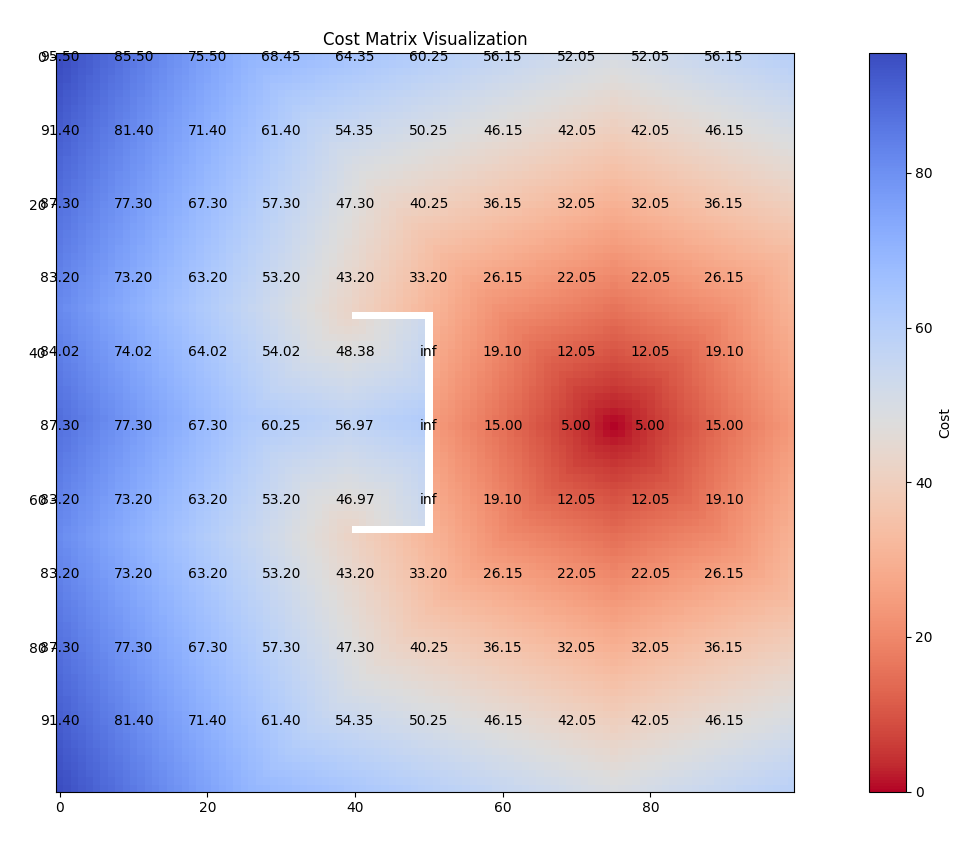
\includegraphics[width=0.9\linewidth]{images/task4_dij_chicken_cost.png}
        \caption{\texttt{cost\_matrix} of Chicken Test}
    \end{subfigure}
    \begin{subfigure}[t]{0.5\textwidth}
        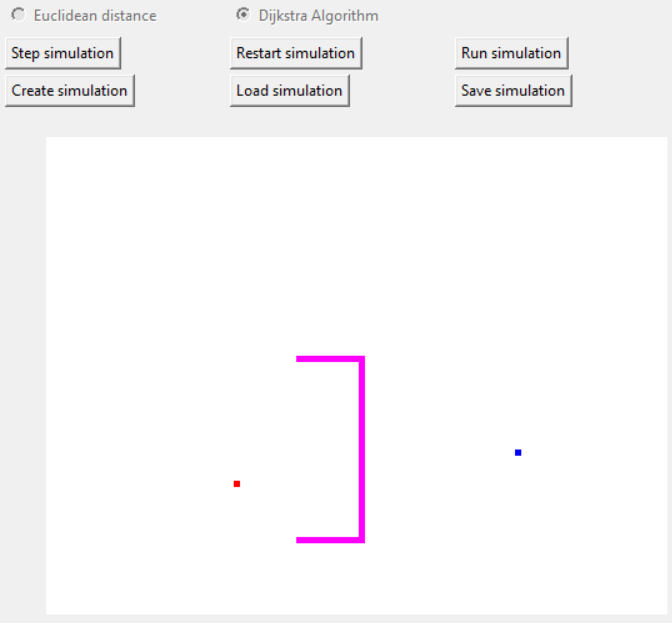
\includegraphics[width=0.9\linewidth]{images/task4_dij_chicken_begin.png}
        \caption{The pedestrian does not move inside of the box \\ but tries to go around it}
    \end{subfigure}
    \begin{subfigure}[t]{0.5\textwidth}
        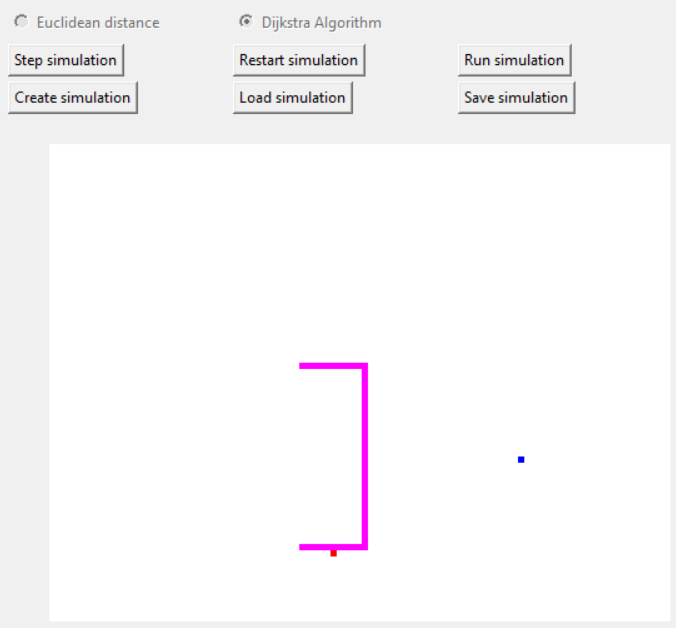
\includegraphics[width=0.9\linewidth]{images/task4_dij_chicken_mid.png}
        \caption{To reach the target with the shortest path, \\ the pedestrian goes close to the obstacle.}
    \end{subfigure}
    \begin{subfigure}[t]{0.5\textwidth}
        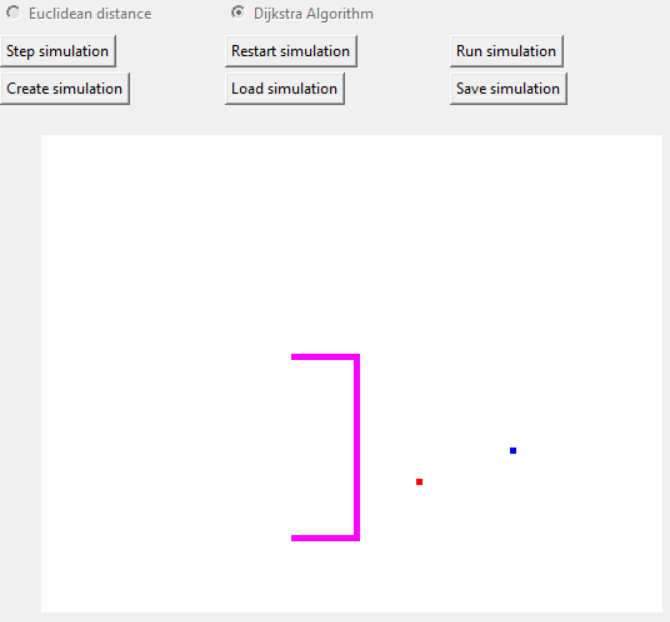
\includegraphics[width=0.9\linewidth]{images/task4_dij_chicken_end.png}
        \caption{Pedestrian tries to come close again to the border line in order to reach the target as quickly as possible using the shortest path.  }
    \end{subfigure}






    
    \caption{Chicken Test using Dijkstra's shortest path algorithm}
    \label{fig:dij_chick}
\end{figure}





\end{task}








\begin{task}{5, Tests}
The guideline "Richtlinie für Mikroskopische Entfluchtungsanalysen" (RiMEA, translation: "Policy
for microscopic evacuation analysis") provides several test scenarios, four of which we will further investigate. \\ 

\textbf{TEST1: RiMEA scenario 1 (straight line):}\\ According to the given test case, It is to be proven that a person in a 2 m wide and 40m long corridor with a defined walking speed will
cover the distance in the corresponding time period.\\
I have initialized one pedestrian at the coordinate (0,20) with the target being at (0,40) and run the simulation.

\begin{figure}[H]
     \centering
     \begin{subfigure}[b]{0.3\textwidth}
         \centering
         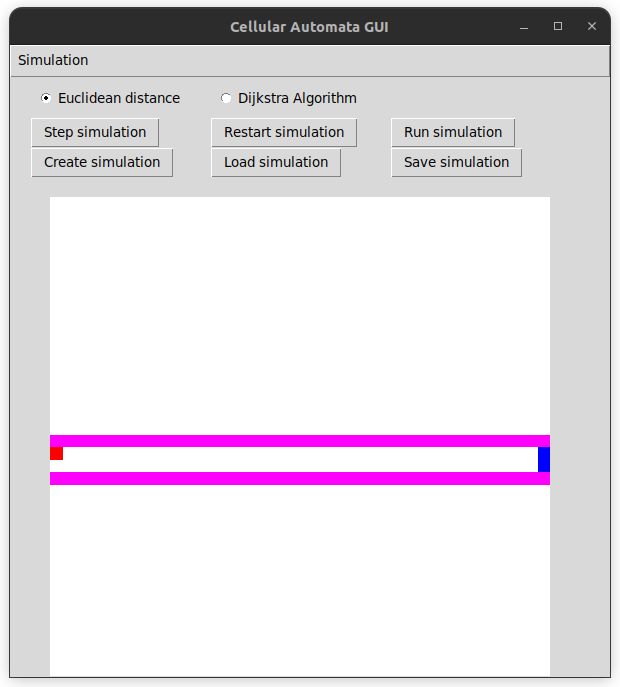
\includegraphics[width=\textwidth]{images/task1_initial.png}
         \caption{Starting position}
         \label{fig:task1_initial}
     \end{subfigure}
     \begin{subfigure}[b]{0.3\textwidth}
         \centering
         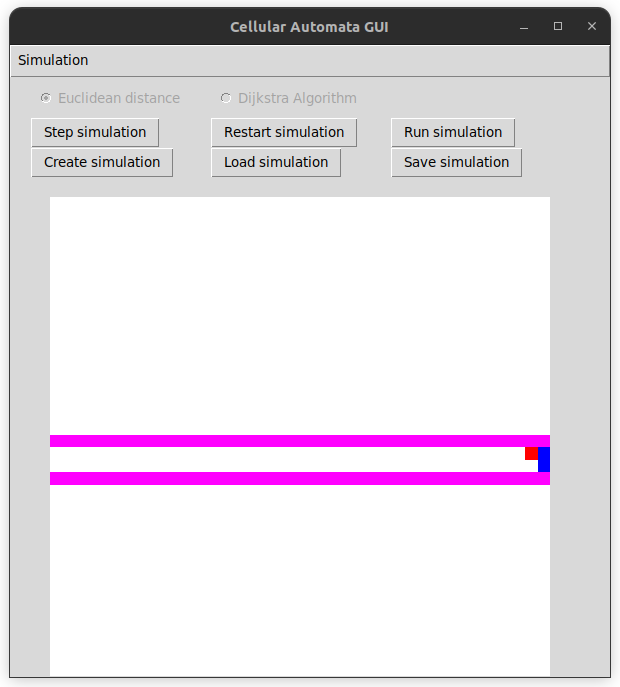
\includegraphics[width=\textwidth]{images/task1_final.png}
         \caption{Final Position} 
         \label{fig:task1_final}
     \end{subfigure}
     \centering
    \caption{RiMEA Scenario 1 (straight line)} 
    \label{fig:task1}
\end{figure}

\ref{fig:task1_initial} shows the initial configuration of task 1. \ref{fig:task1_final} shows the final position of the pedestrian being absorbed by the target. The pedestrian reaches the target in \begin{tt}
    39.0 seconds
\end{tt} with a speed of \begin{tt}
    1.0 m/s.
\end{tt}\\

\textbf{TEST2: RiMEA scenario 4 (fundamental diagram: density vs. velocity or density vs. flow):}\\

For this scenario, we had a corridor of 5x275 meters and put different densities of people here for testing. We put different numbers of pedestrians in this corridor; however, as we increased the density, our computers could not handle the simulation. Like in the Figure \ref{fig:task5_scenario4}.\\

\begin{figure}[H]
    \centering
    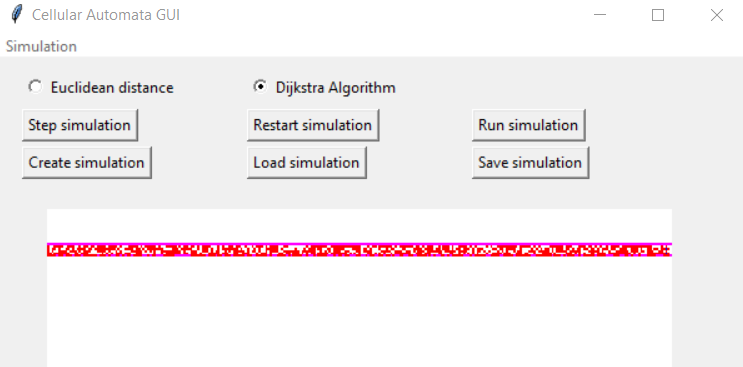
\includegraphics{images/task5_scenario4.png}
    \caption{1370 people put inside of a corridor}
    \label{fig:task5_scenario4}
\end{figure}

Therefore, instead of using all control points, we used only the ones near to target points with a much smaller number of pedestrians. We got some results, but they were not as expected. Our implementations were fine in other scenarios but in this one, we got erroneous values. \\

Basically, at the control points, our code tries to find the average speed values of pedestrians going through that point and we store these values inside of \texttt{self.speeds225\_18, self.speeds250\_17, self.speeds250\_18 } variables, depending on their location. After getting the average speed for each second, we store this information inside of \texttt{total\_speeds225\_18, total\_speeds250\_17, total\_speeds250\_18} attributes. In the end, we just take the average of the average speeds at each second. Then, print them on the console. Although the results were erroneous most probably due to some mistakes in our implementation, the simulation seemed to be running correctly.\\

To avoid creating many pedestrians with random attributes by hand, we created and used \texttt{pedestrian\_generator.py}. 



\textbf{TEST3: RiMEA scenario 6 (movement around a corner):}\\
In the RiMEA test scenario 6, a 2m wide corridor with a corner is to be modeled, which can be seen in figure \ref{fig:rimea6a}. The file \verb|RiMEA6.json| provides the corresponding setup, where 4 grid cells equal 1 square meter. Figure \ref{fig:rimea6b} and \ref{fig:rimea6c} show the process of the pedestrians walking to the right side before moving up to the target in order to avoid the obstacle. Without the obstacle, the pedestrians are able to move diagonally and thus reach the target faster. 

\begin{figure}[H]
     \centering
     \begin{subfigure}[b]{0.3\textwidth}
         \centering
         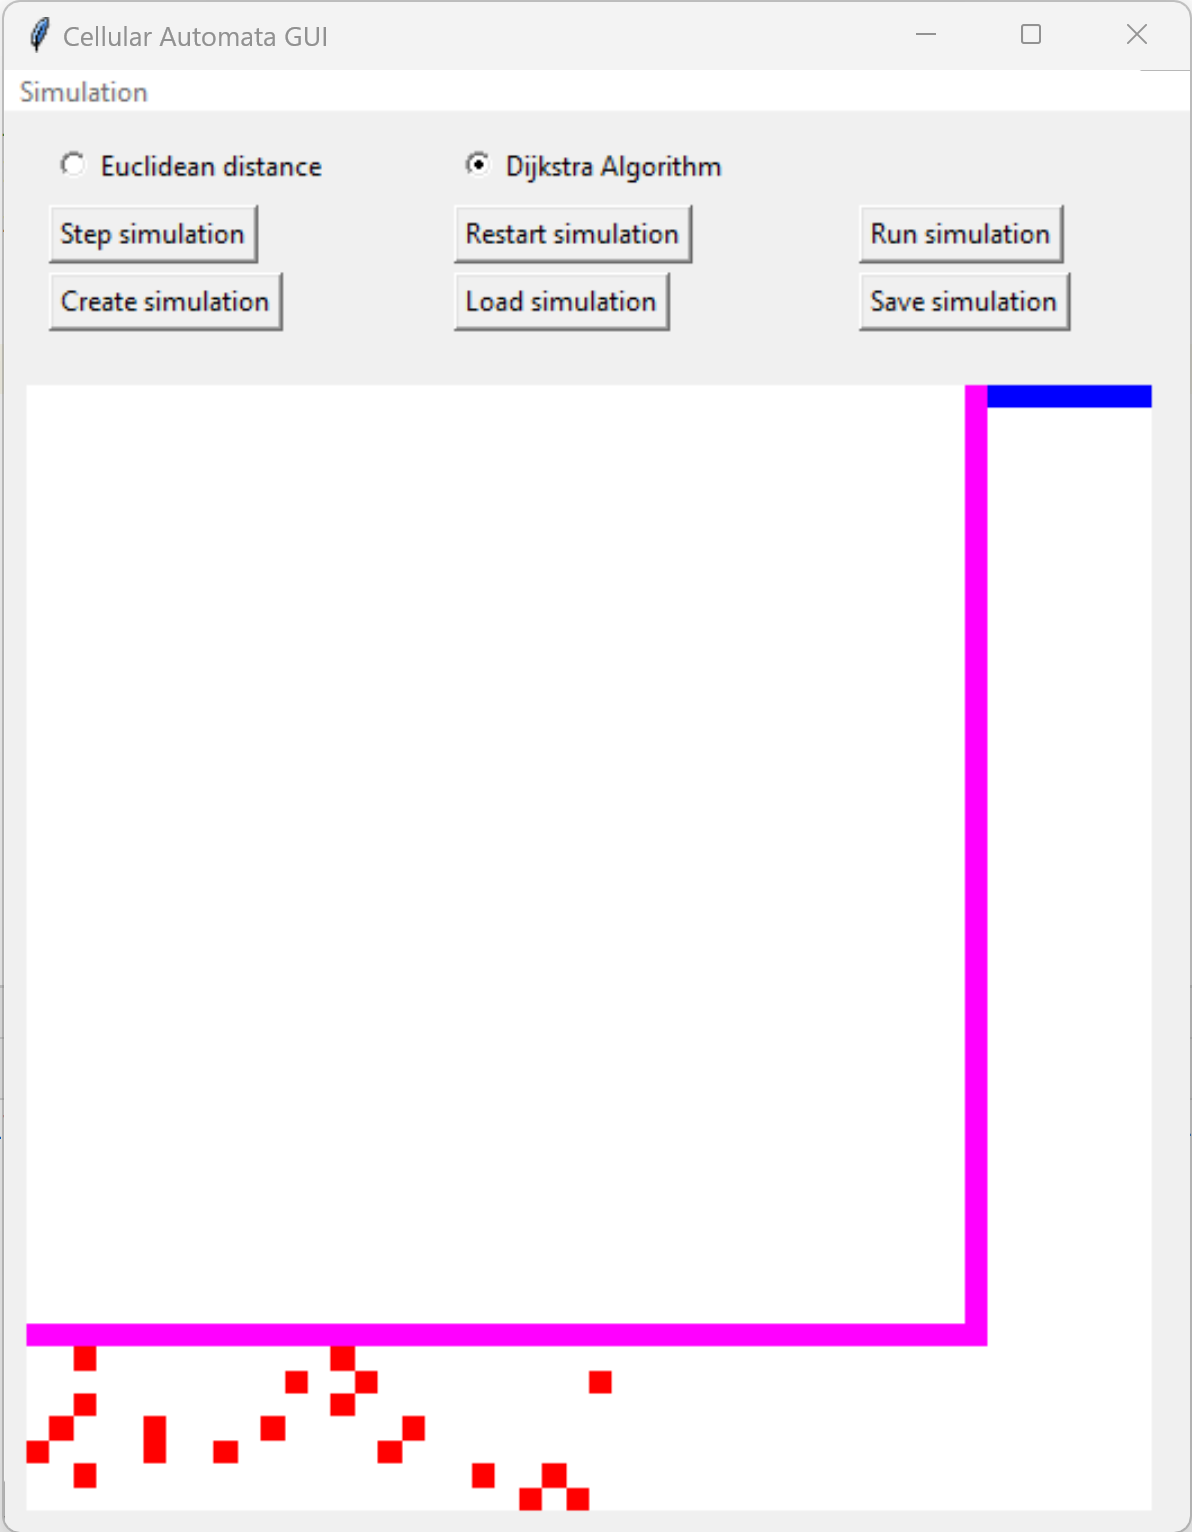
\includegraphics[width=\textwidth]{images/1-rimea6.png}
         \caption{Starting position}
         \label{fig:rimea6a}
     \end{subfigure}
     \begin{subfigure}[b]{0.3\textwidth}
         \centering
         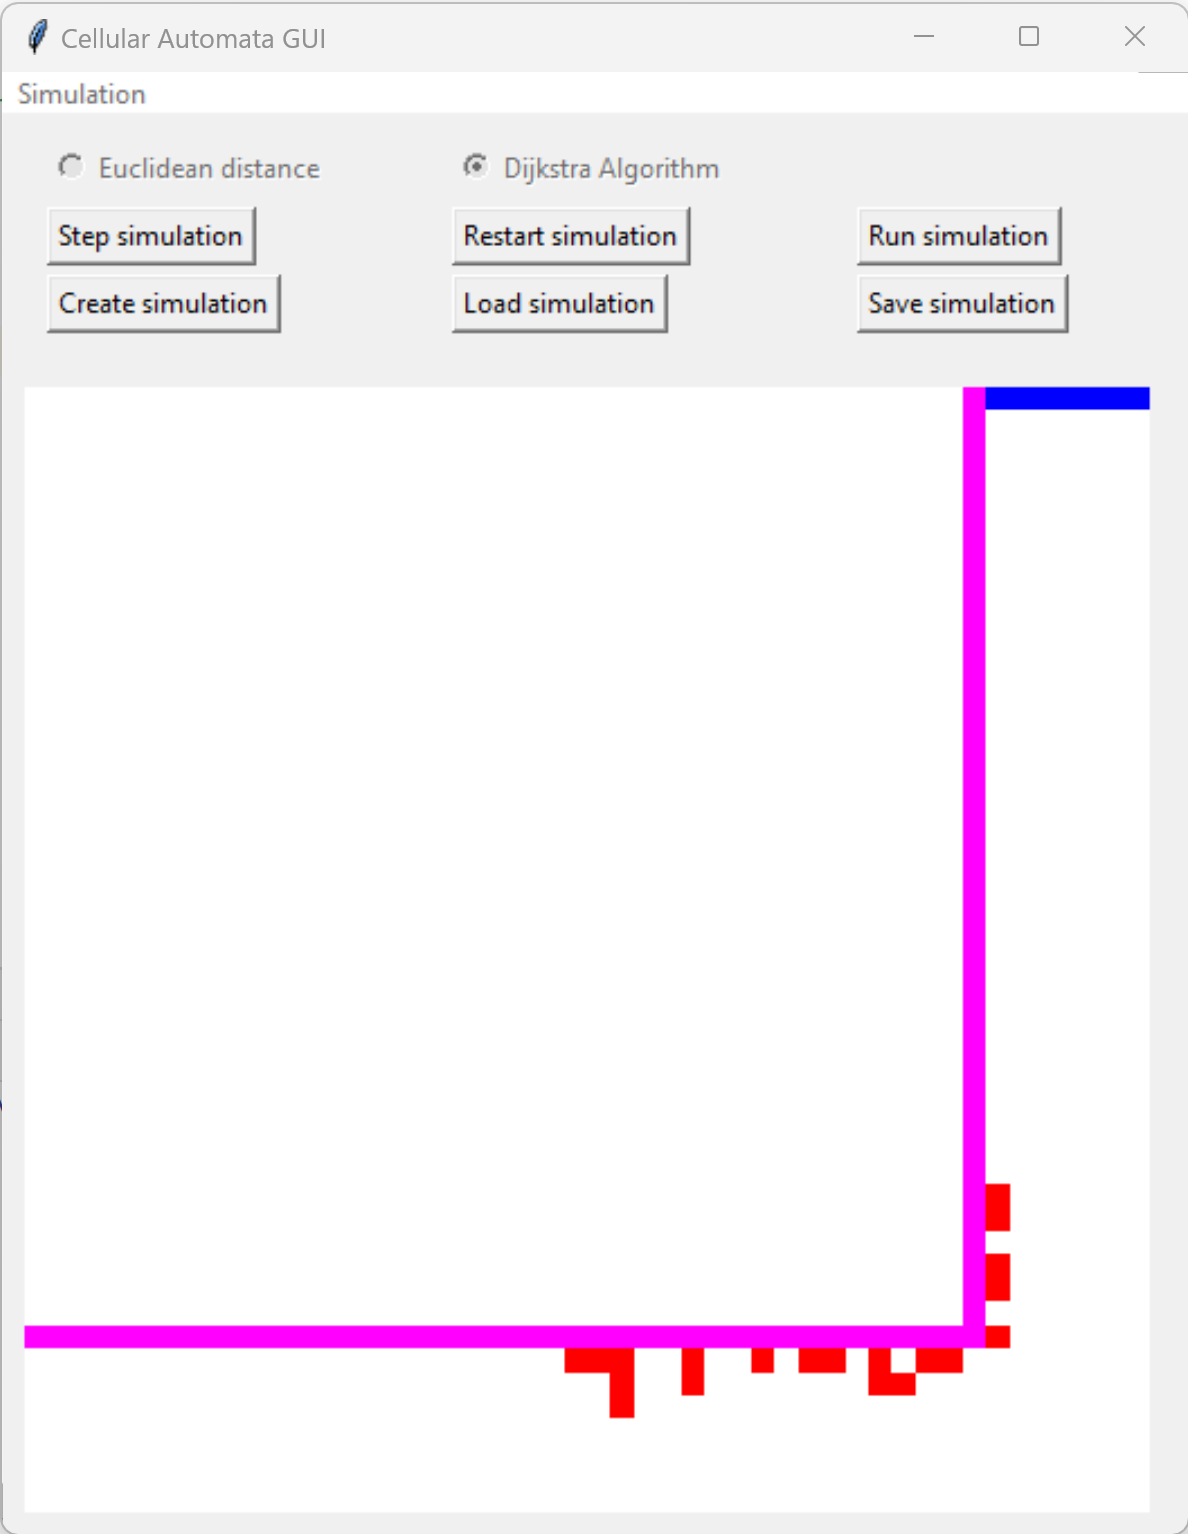
\includegraphics[width=\textwidth]{images/1-rimea6b.png}
         \caption{Process}
         \label{fig:rimea6b}
     \end{subfigure}
     \centering
     \begin{subfigure}[b]{0.3\textwidth}
         \centering
         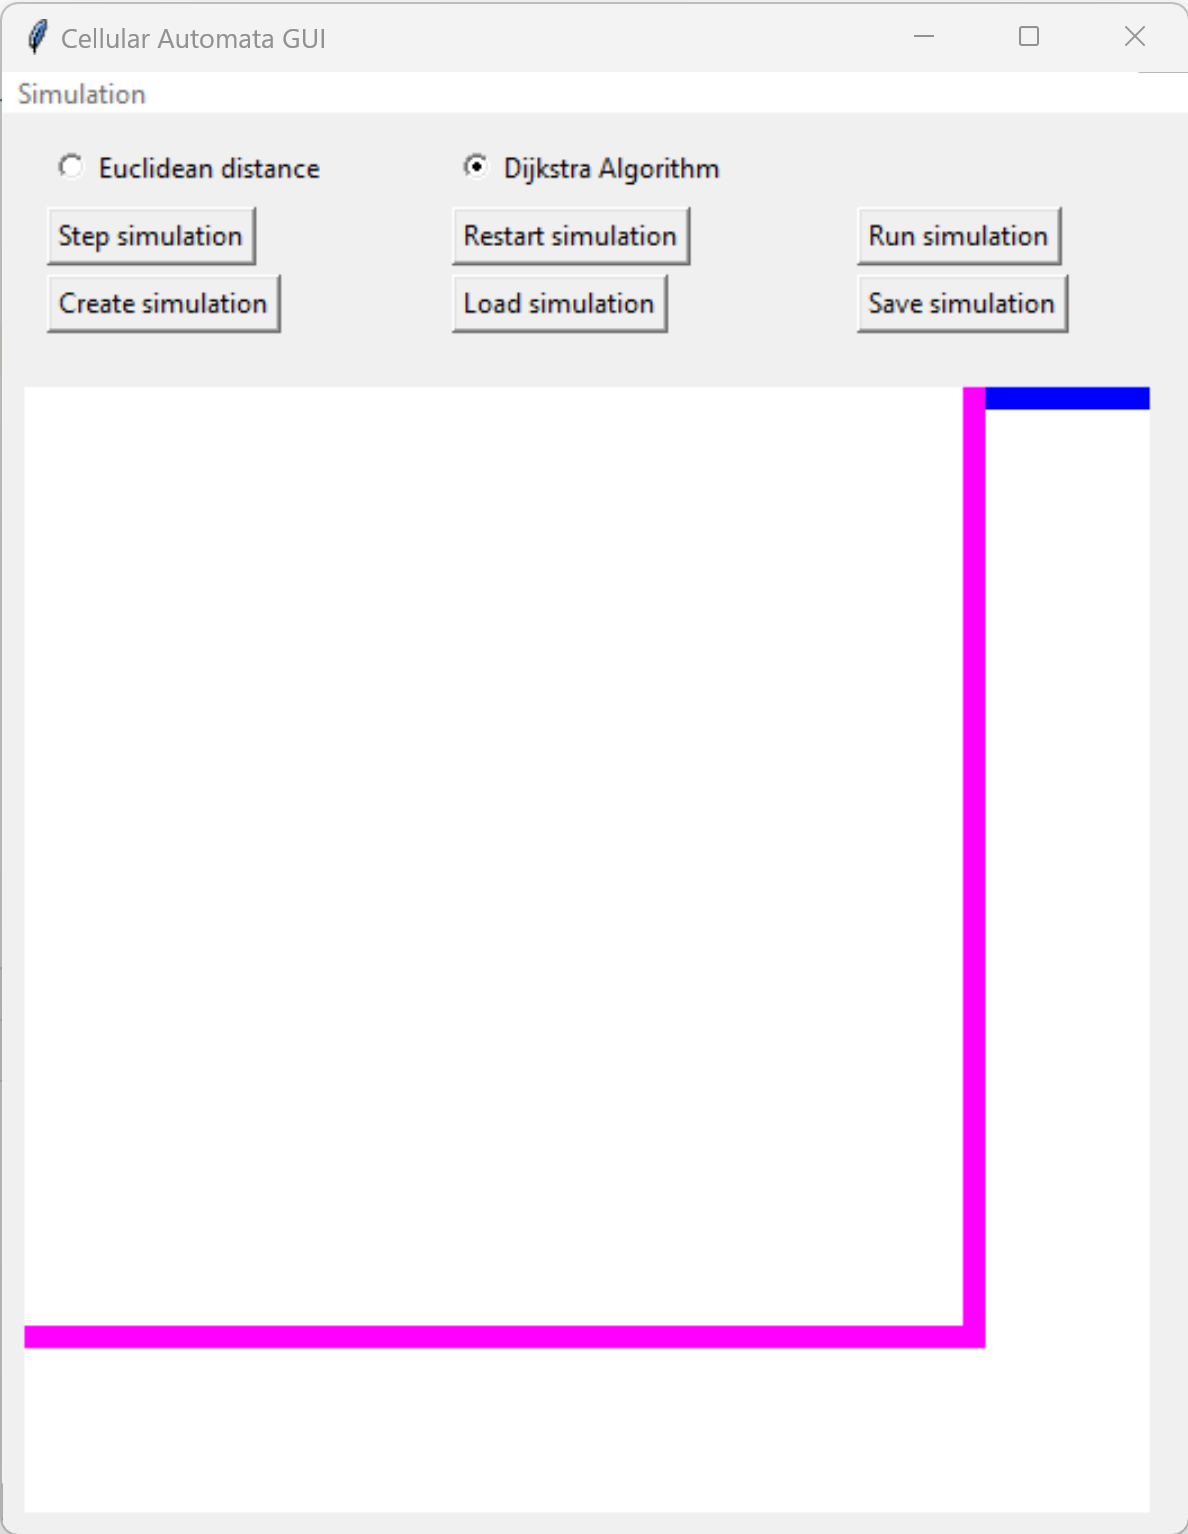
\includegraphics[width=\textwidth]{images/1-rimea6c.png}
         \caption{Target position}
         \label{fig:rimea6c}
     \end{subfigure}
    \caption{In RiMEA scenario 6, the pedestrians move around a corner}
    \label{fig:rimea6}
\end{figure}

\textbf{TEST4: RiMEA scenario 7 (demographic parameters):}\\
In this test, we have to consider 50 pedestrians with varying walking speeds distributed according to walking speed distributions described in Figure 2 of the RiMEA document \cite{RiMEA}. In order to do this we generated speeds for different age groups sampled from the estimates based on the figure, as outlined in Table \ref{table:speedTable}.


\begin{table} [H]
\centering
\begin{tabular}{|c|c|c|c|}
\hline
Age group & Number of pedestrians & Min Speed [m/s] & Max Speed [m/s] \\
\hline
0-10 & 5 & 0.60 & 1.20 \\
10-20 & 5 & 1.20 & 1.60 \\
20-40 & 10 & 1.50 & 1.60 \\
40-50 & 10 & 1.40 & 1.50 \\
50-60 & 10 & 1.30 & 1.40 \\
60-70 & 5 & 1.10 & 1.30 \\
70-80 & 5 & 0.60 & 1.10 \\
\hline
\end{tabular}
\caption{Speed distribution as per age}
\label{table:speedTable}
\end{table}


Figure \ref{fig:rimea7a} demonstrates the initial position of all the pedestrians starting from the same column with targets being located at the other end. After running the simulation for some time, we can see that in figure \ref{fig:rimea7b} different age groups form different movement groups corresponding to their walking speeds. The outcome aligns with the movement patterns outlined in the RiMEA document.\cite{RiMEA} The statistical values have also been saved in the \begin{tt}
    statistics.json
\end{tt} file for further investigation.


\begin{figure}[H]
     \centering
     \begin{subfigure}[b]{0.3\textwidth}
         \centering
         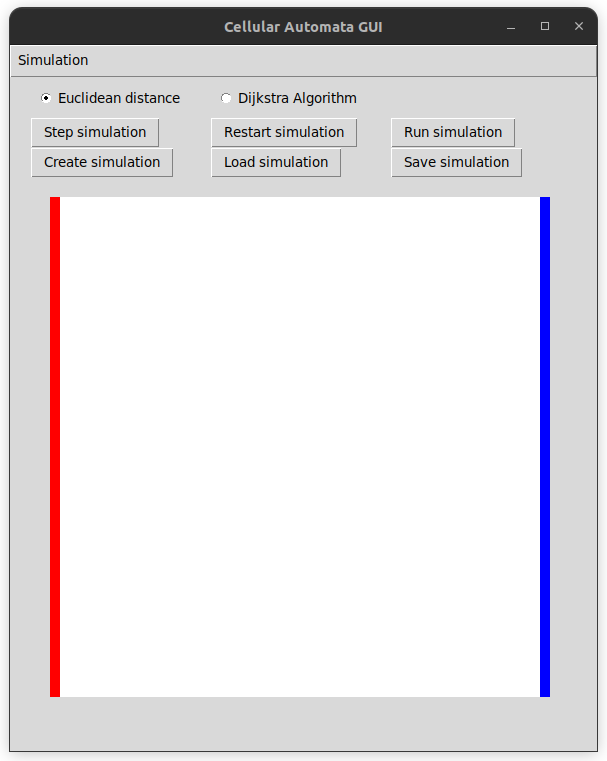
\includegraphics[width=\textwidth]{images/scenario7_initial.png}
         \caption{Starting position}
         \label{fig:rimea7a}
     \end{subfigure}
     \begin{subfigure}[b]{0.3\textwidth}
         \centering
         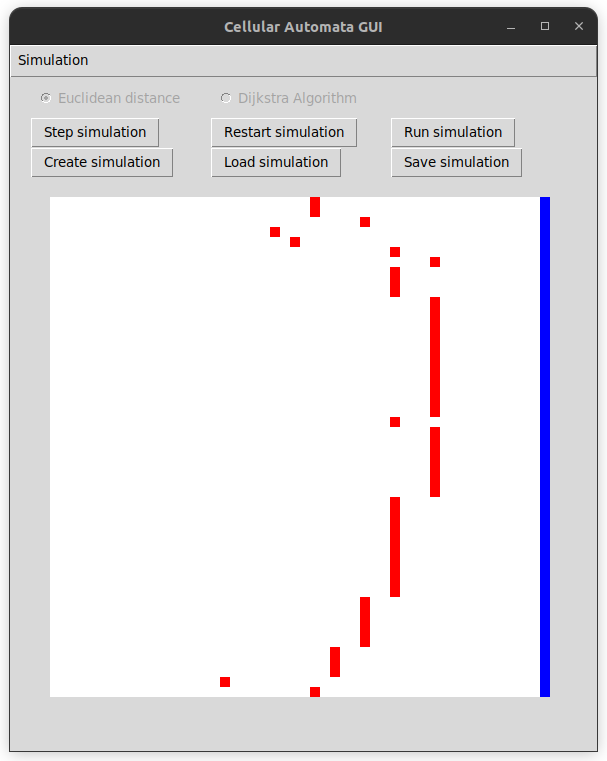
\includegraphics[width=\textwidth]{images/scenario7_middle.png}
         \caption{Process}
         \label{fig:rimea7b}
     \end{subfigure}
    \caption{The different age groups can be seen forming a movement group }
    \label{fig:rimea7}
\end{figure}
\end{task}

\bibliographystyle{plain}
\bibliography{Literature}

\end{document}